\subsection{System identification and identification signal}
\label{sec:Results_ident}
As discussed, the desired area of interest for this thesis is the up-up configuration of the ADIP. To this end, a closed-loop feedback controller is designed for the local model, which tracks a reference trajectory. The tracking data, which comprises state and input measurements, is then used as the raw data to approximate a data-driven controller. Additionally, Brunton et al. \cite{SINDyc}, and Kaiser et al. \cite{kaiser2020datadriven} observe that during closed-loop identification since the feedback is a function of the state, there is a need to add sufficiently large white noise or kick the system occasionally with large impulse or step inputs to distinguish the feedback dynamics of the input from the state dynamics. Note that this step is not necessary for open-loop system identification, which will be discussed later.\par
In this thesis work, a reference trajectory, as shown in Figure \ref{fig:ReferenceTraj} was chosen for which an LQ regulator was designed. The resulting input signal is shown in Figure \ref{fig:InputSignal}. This input signal is the feedback signal perturbed by a white noise of noise power 0.05. \\
\begin{figure}[ht]
    \captionsetup[subfigure]{justification=centering}
    \centering
    \begin{subfigure}[t]{1\textwidth}
    \centering
    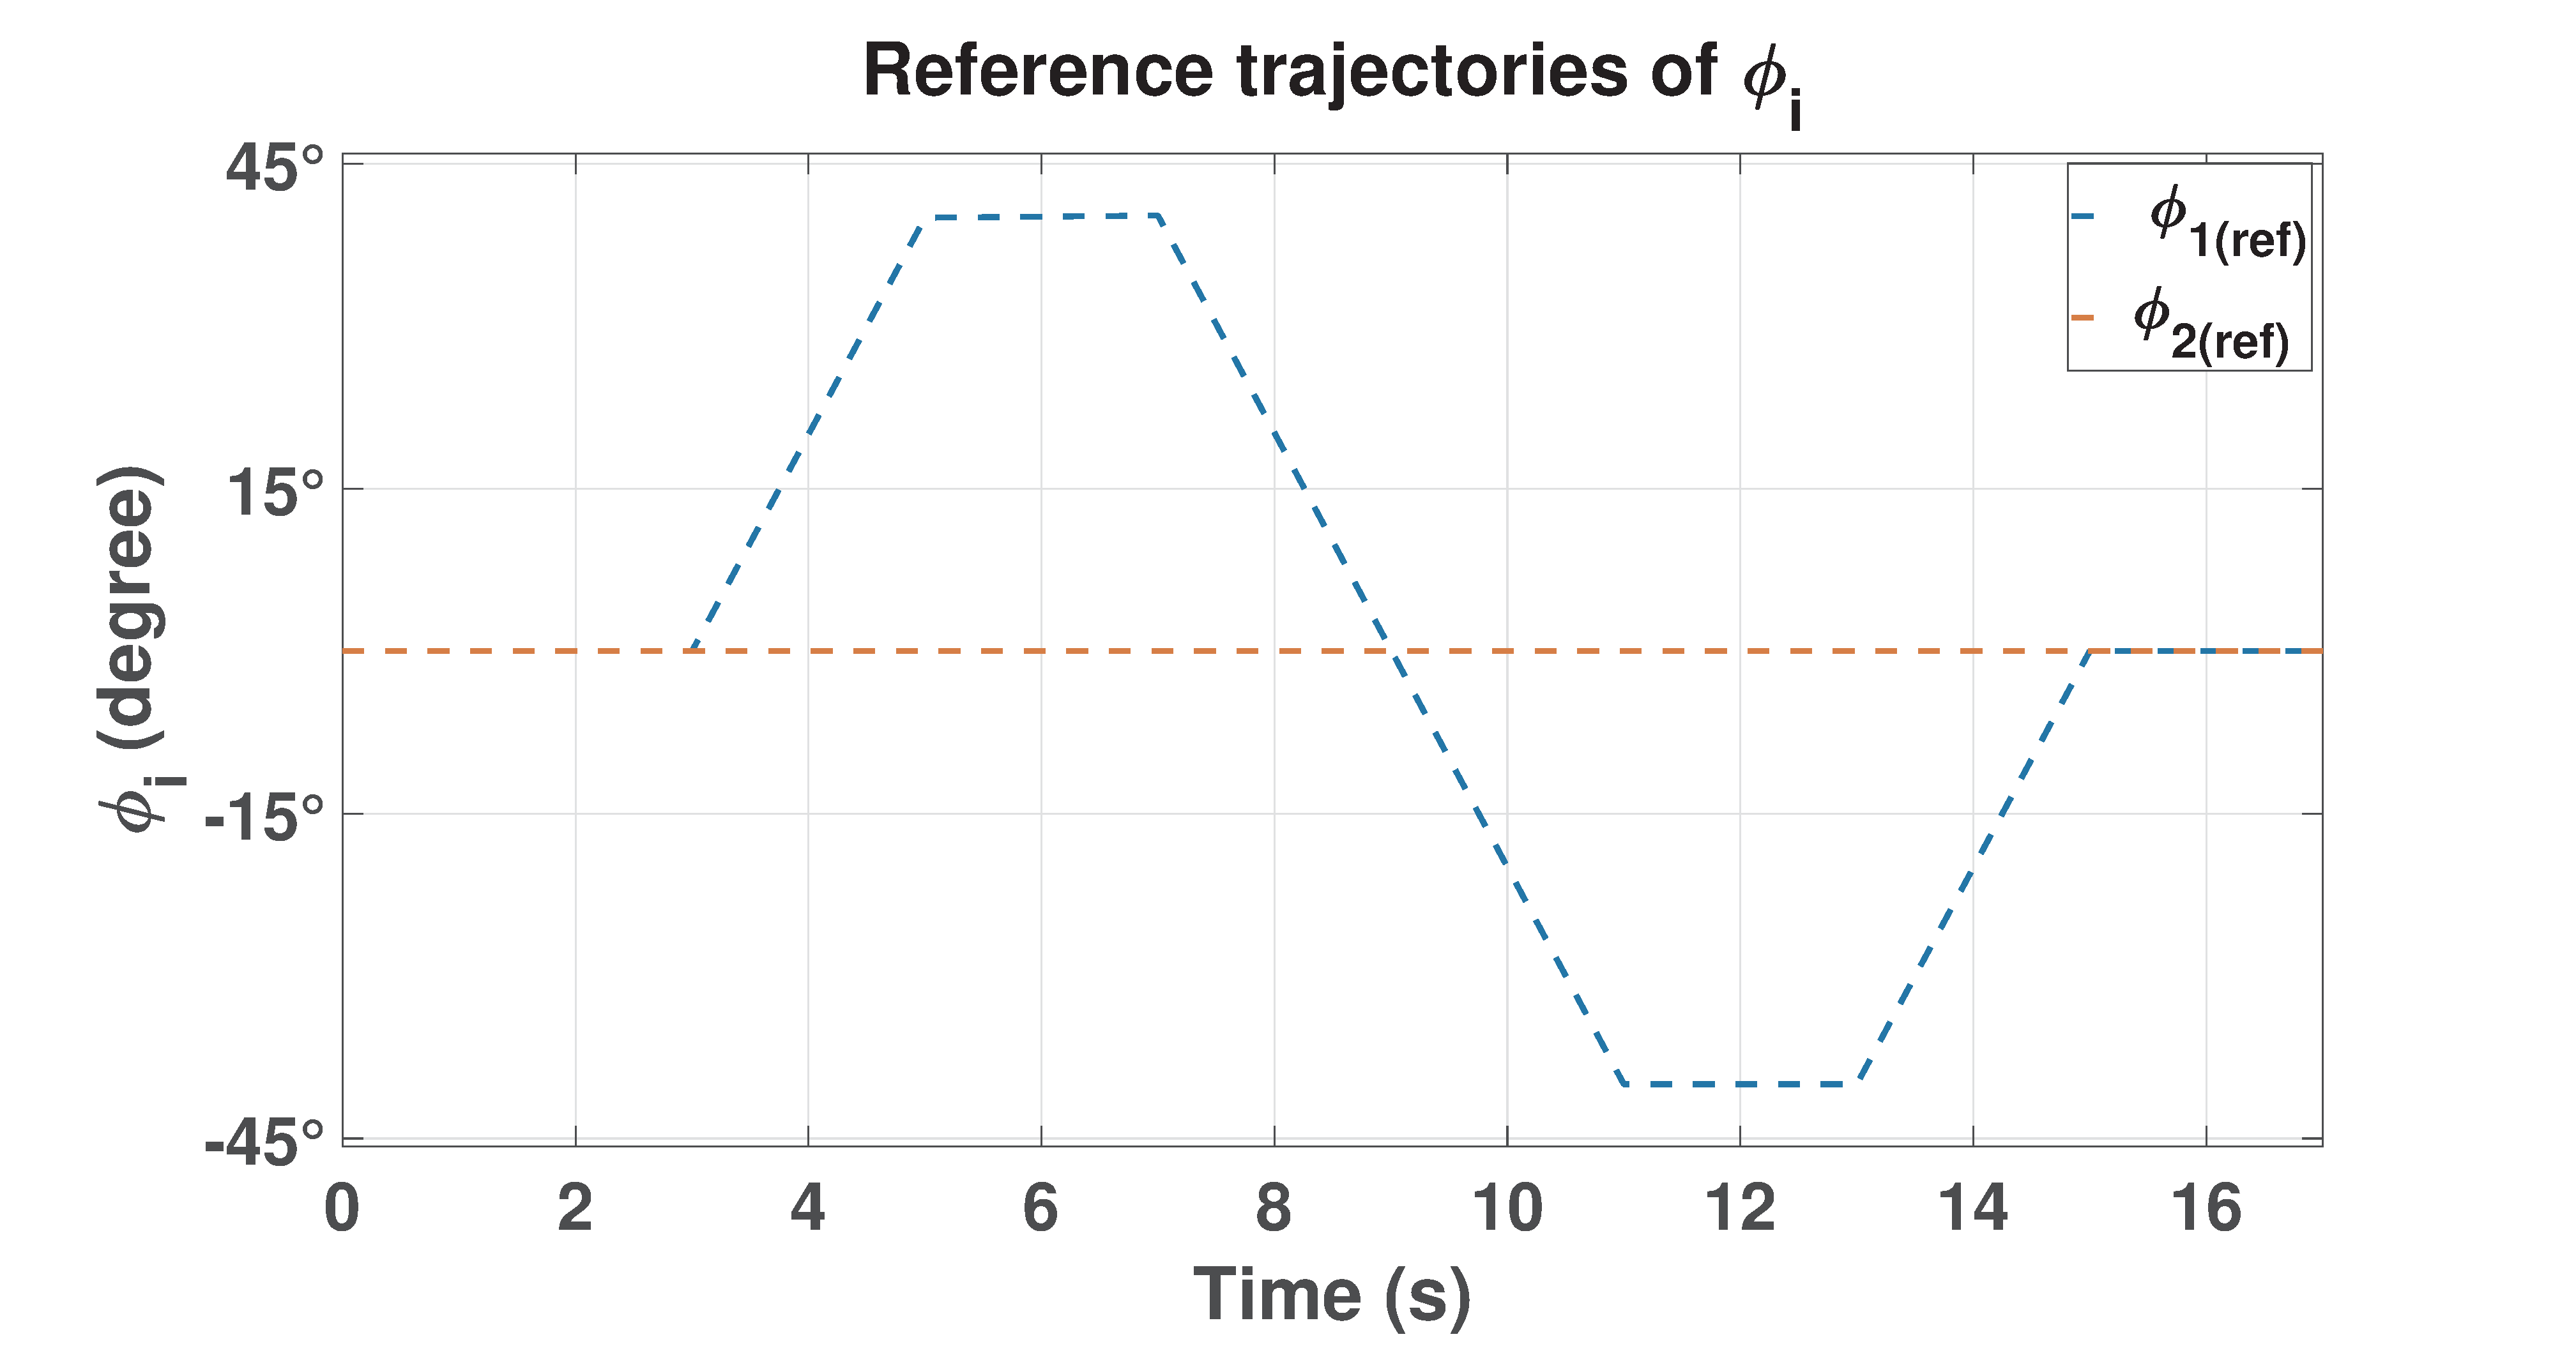
\includegraphics[width=1\linewidth]{figures/Reference}
    \caption{Reference trajectory of the states ($\phi_1$ and $\phi_2$).}
    \label{fig:ReferenceTraj}
    \end{subfigure}%
    \vspace{0.5em}
    \begin{subfigure}[t]{0.485\textwidth}
    \centering
    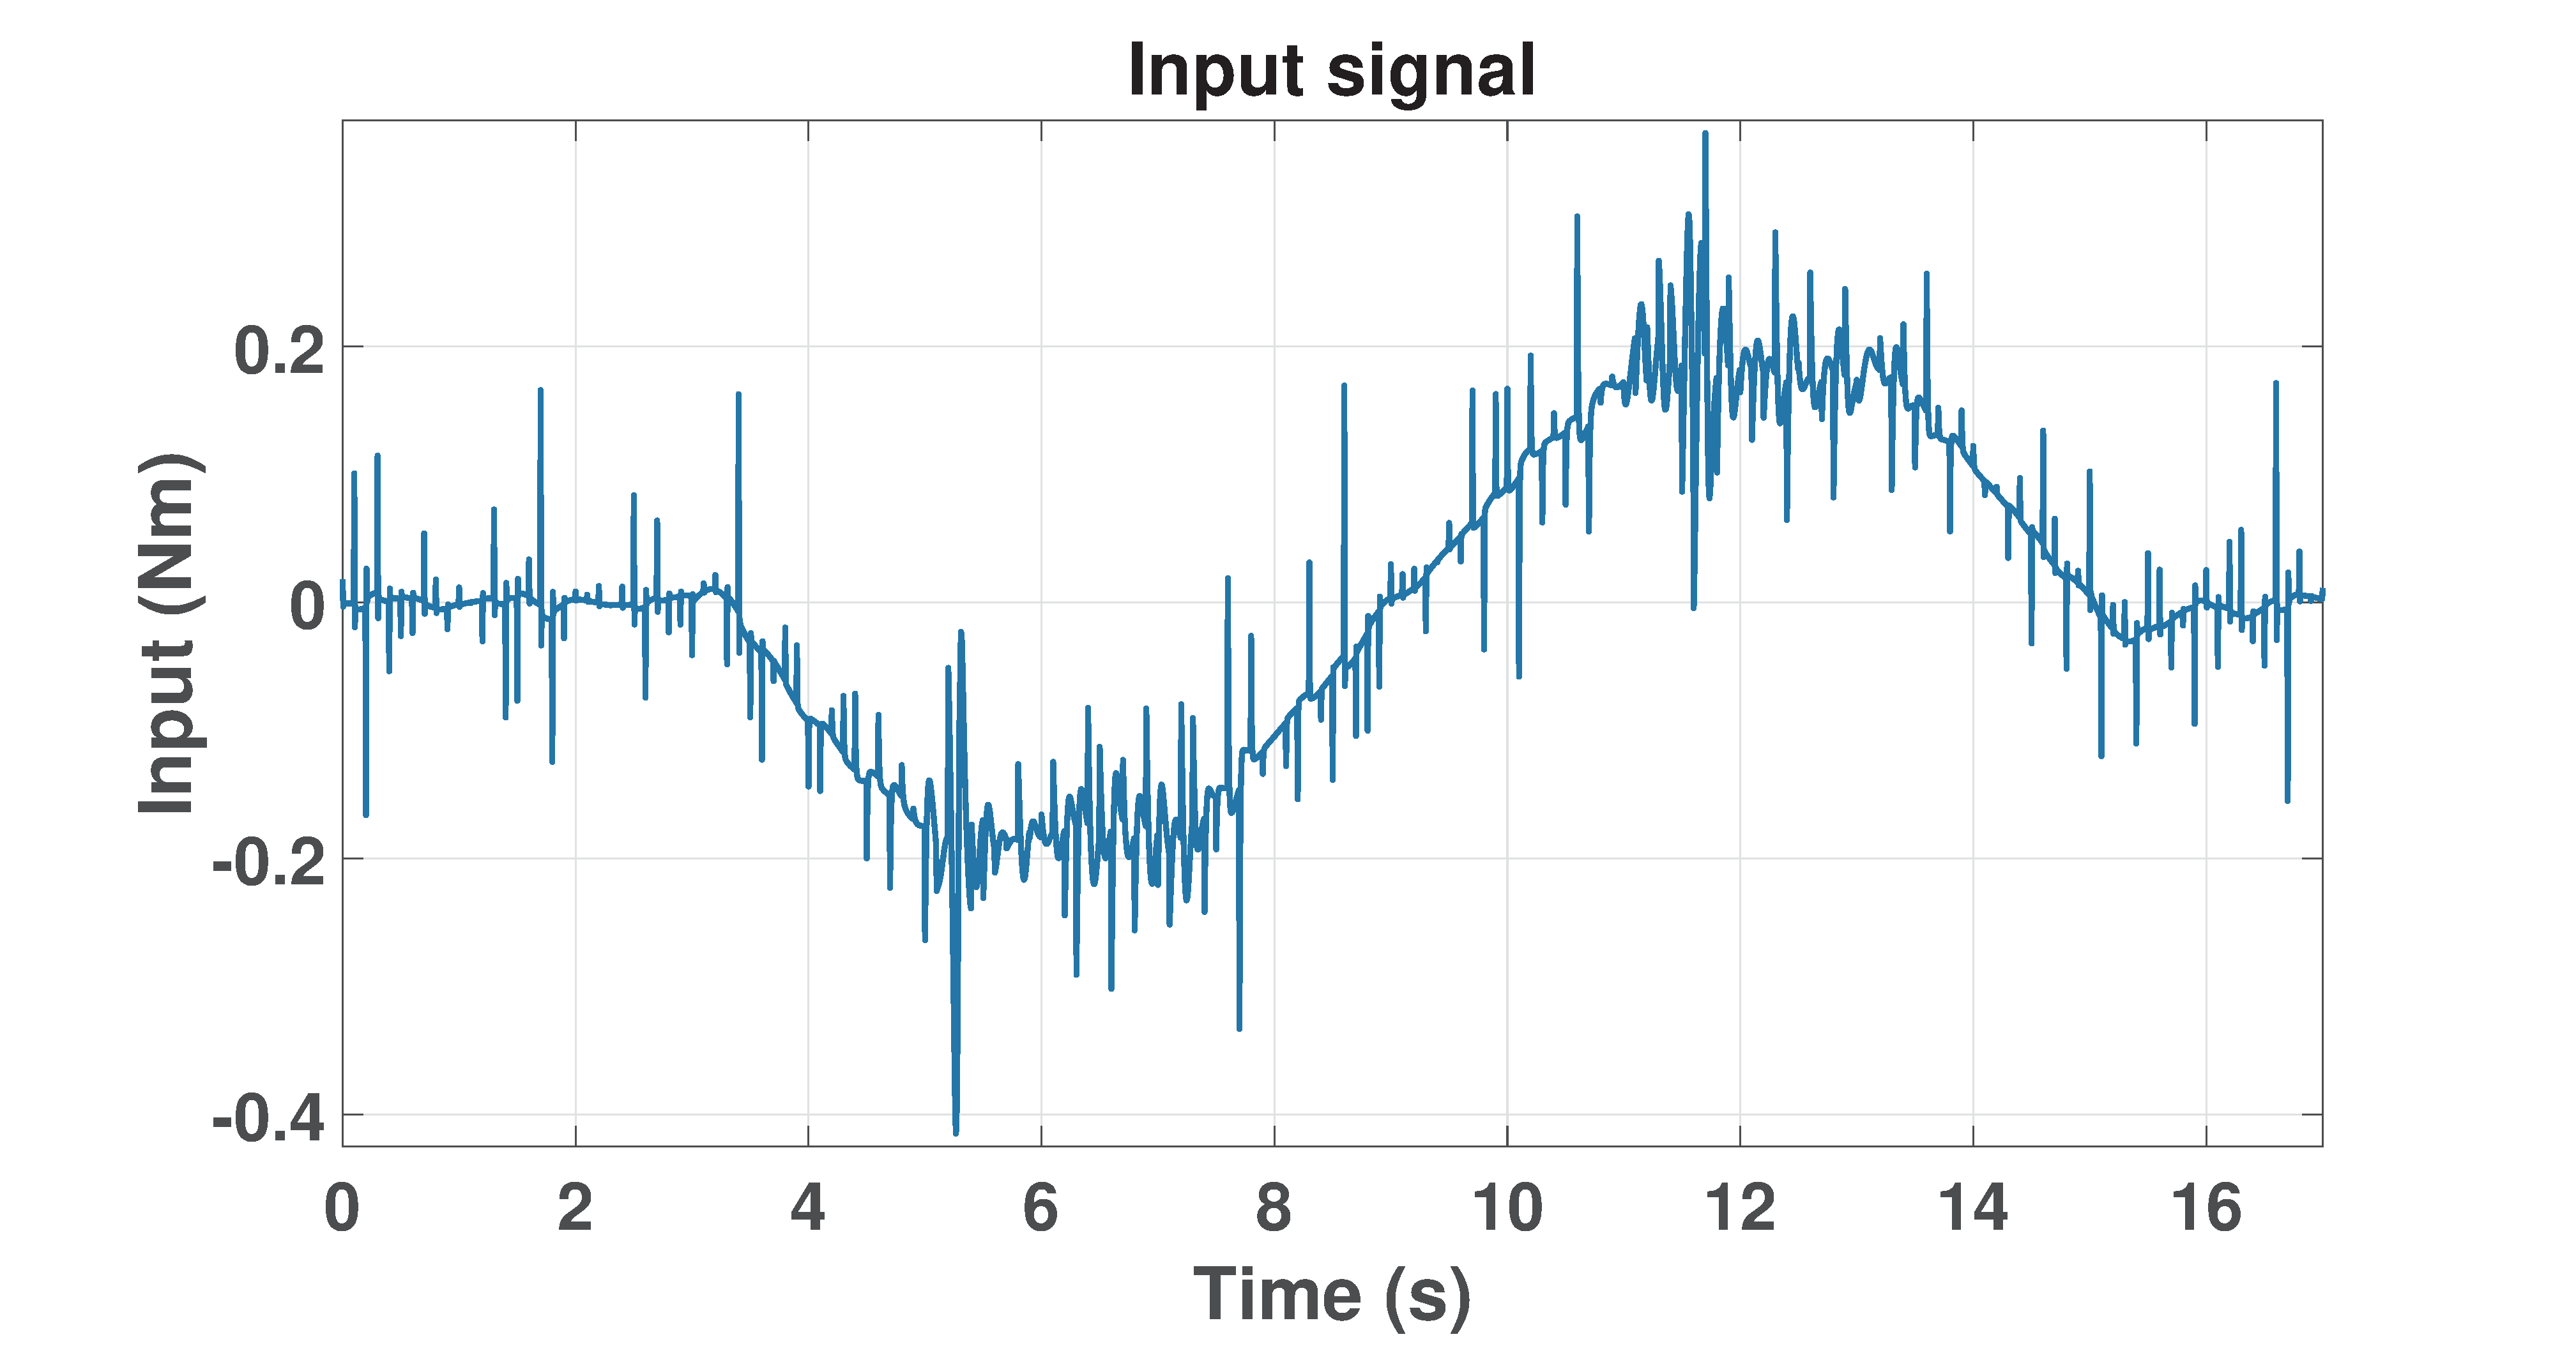
\includegraphics[width=\textwidth]{figures/RefInput}
    \caption{Input signal}
    \label{fig:InputSignal}
    \end{subfigure}
    ~
    \begin{subfigure}[t]{0.485\textwidth}
    \centering
    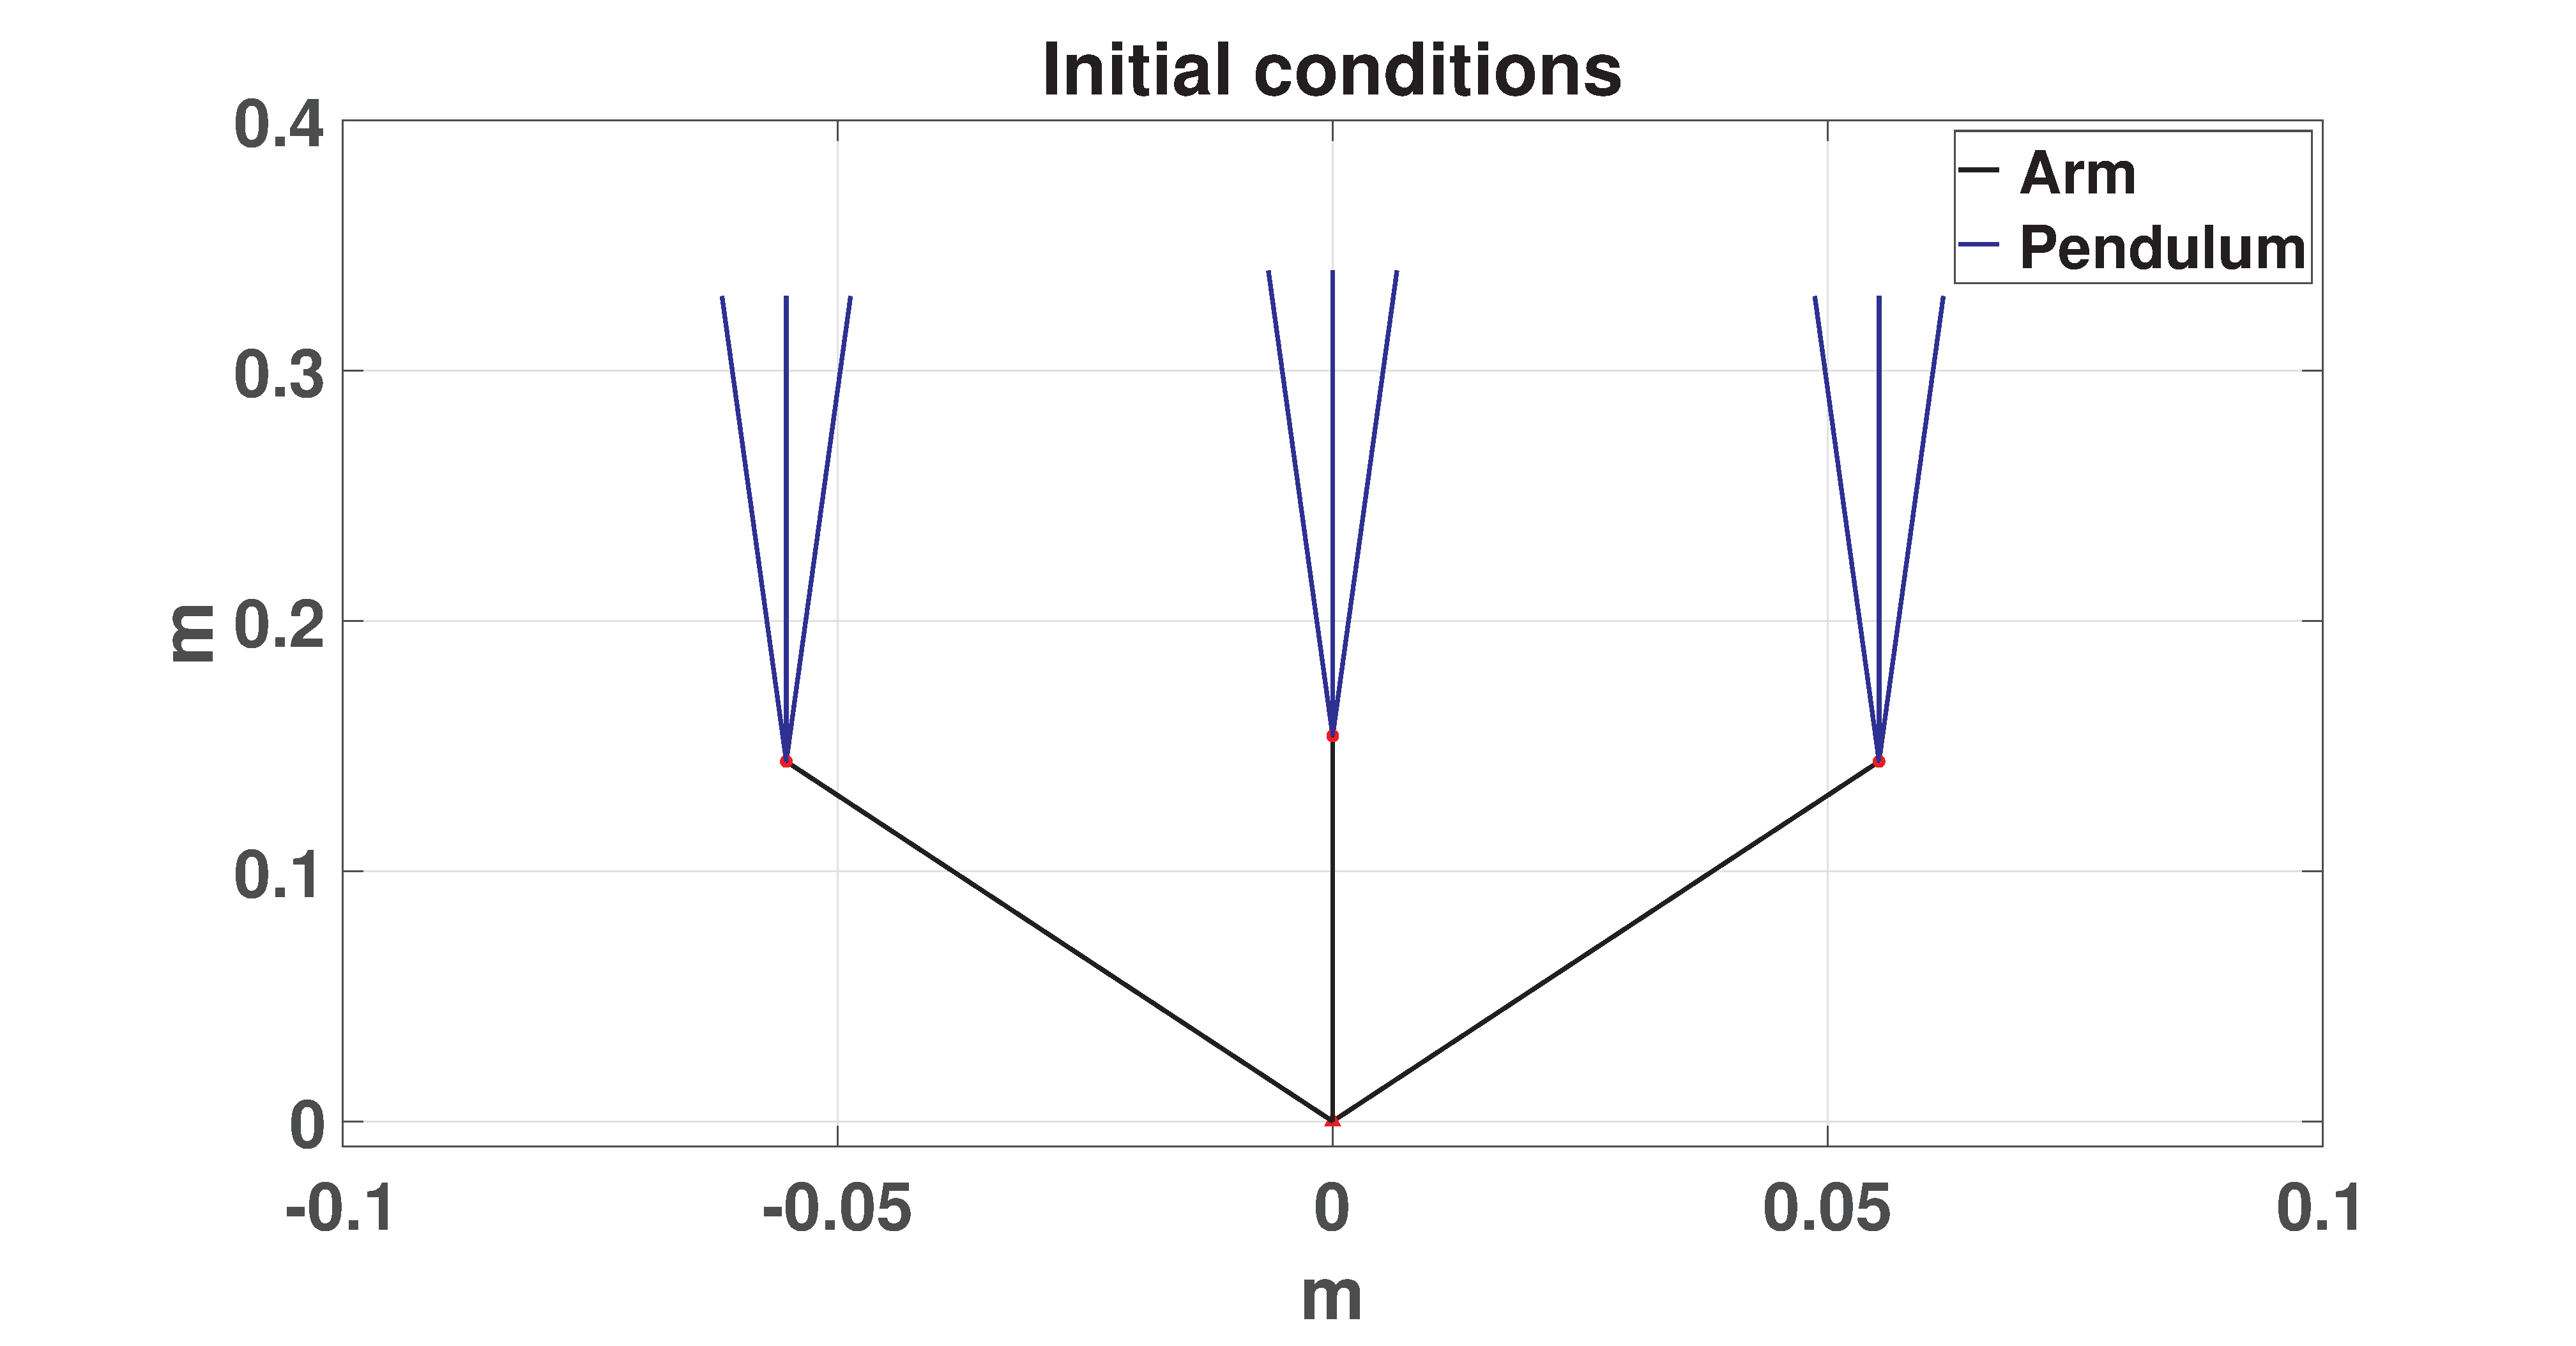
\includegraphics[width=\textwidth]{figures/InitCondn}
    \caption{Visualization of the initial conditions}
    \label{fig:InitCondns}
    \end{subfigure}
    \caption{Reference trajectory, Input signal and Initial conditions}
\end{figure}
\newpage
Data was collected by simulating the system multiple times in closed-loop with random initial conditions given by
\begin{equation}
\label{Eq:MultInit}
    \mathbf{x}_0 = [\mathcal{U}(-1 \quad 1)l_{\phi_1},~\mathcal{U}(-1 \quad 1)l_{\phi_2},~\mathcal{U}(-1 \quad 1)l_{\dot{\phi}_1},~\mathcal{U}(-1 \quad 1)l_{\dot{\phi}_2}] \;,
\end{equation}
where~ $\mathcal{U}(-1,~1)$ is a uniformly distributed random variable with range $-1$ to $1$, and $l_{\phi_1} = 40^{\circ}$, $l_{\phi_2} = 2^{\circ}$, $l_{\dot{\phi}_1} = l_{\dot{\phi}_2} = 0.25$rad/s. Therefore, the initial condition is uniformly distributed around the unstable equilibrium ($\phi_1 = \phi_2 = \dot{\phi}_1 = \dot{\phi}_2 = 0^{\circ}$) and its range is defined by $L = [l_{\phi_1}, l_{\phi_2}, l_{\dot{\phi}_1}, l_{\dot{\phi}_2} ]$. Figure \ref{fig:InitCondns} visualizes the distribution of initial conditions with respect to the states $\phi_1$ and $\phi_2$. $L$ was chosen by trial-and-error and it represents the range limit in which the controller is able to track the subsequent reference trajectory successfully. One might also choose $L$ by evaluating a regulation task instead of tracking. The data was generated by simulations of 17s each on a nonlinear model of the ADIP (refer Chapter \ref{Chapter:Plant}) where the controller tracked the reference trajectory~(Fig.~\ref{fig:ReferenceTraj}). The data was sampled every 5ms. The subsequent approximation of the linear matrices follows the procedure detailed in Section \ref{sec:EDMD}. \par
As stated previously, although the region of interest for this thesis work is the up-up configuration for which only closed-loop identification is possible, open-loop identification around the stable equilibrium nevertheless presents numerous important insights into the generation of data and choice of observables, which was then applied to generate data and/or influenced the choice of observables in closed-loop identification. During the course of this thesis, numerous combinations of observables and data were tried and analyzed, and this could not have been easily done in the up-up configuration as it demands a corresponding controller to stabilize the system.\par
In this thesis, SINDy with control (SINDYc) algorithm (refer Section \ref{sec:SINDy}) is used to approximate the open-loop dynamics to demonstrate the working of SINDy algorithm. EDMDc can also very well be used for the same. However, SINDYc approximates the states' time evolution directly from data and a set of candidate functions without having to go through the hassle of choosing the `correct' observables and computing the corresponding Koopman operator. It is important to note that SINDYc has also been used for feedback control of nonlinear systems \cite{SINDyc}; however, this has not been implemented in this work.\par
The forcing function used in open-loop identification is a chirp signal with the frequency defined in the range $[f_{min}~ f_{max}]$ and with amplitude $A$. The frequencies and amplitudes were chosen such that the system does not translate to the `chaotic zone' but is also sufficiently perturbed away from its stable equilibrium. The chirp signal can be generated using the \textit{chirp} command in Matlab. In summary, the forcing functions for training and validation purposes are given as,
% 
\begin{align}
\label{Eq:Forcing}
\begin{split}
    \textup{Training} &\rightarrow A*chirp(t,f_{min},t_s,f_{max},[~],-90), \quad [f_{min}~f_{max}] = [0.3 ~ 0.7]\textup{Hz}, A = 0.1 \;, \\ 
    \textup{Validation} &\rightarrow A*chirp(t,f_{min},t_s,f_{max},[~],-90), \quad [f_{min}~f_{max}] = [0.7 ~ 0.9]\textup{Hz}, A = 0.065 \;.
\end{split}
\end{align}
% 
First, the case for data obtained from multiple trajectories is made. As Abraham et al. \cite{Abraham} observed, the number of data points and their distribution across the state space will have a large effect on the computed Koopman operator of the underlying nonlinear system. It is always beneficial to record trajectories from multiple initial conditions as shown in (\ref{Eq:MultInit}).\par
Figures \ref{fig:SingleTrajTrain} and \ref{fig: MultTrajTrain} compare the identification of the system through SINDYc from training data generated by a single initial condition and training data generated from multiple initial conditions respectively. The training data generated from multiple initial conditions is visualized in Figure \ref{fig:TrainingData}. In this case, the training data is generated from multiple initial conditions (\ref{Eq:MultInit}) with $l_{\phi_1} = 210^{\circ}$, $l_{\phi_2} = 150^{\circ}$, $l_{\dot{\phi}_1} = l_{\dot{\phi}_2} = 1$rad/s and the forcing function~(\ref{Eq:Forcing}) with $f_{min} = f_{max} = 0.5$Hz and $A = 0.1$, respectively. Again, the choice of these values are influenced by the requirement for trajectories to lie in the non-chaotic zone.
\begin{figure}[ht]
    \centering
    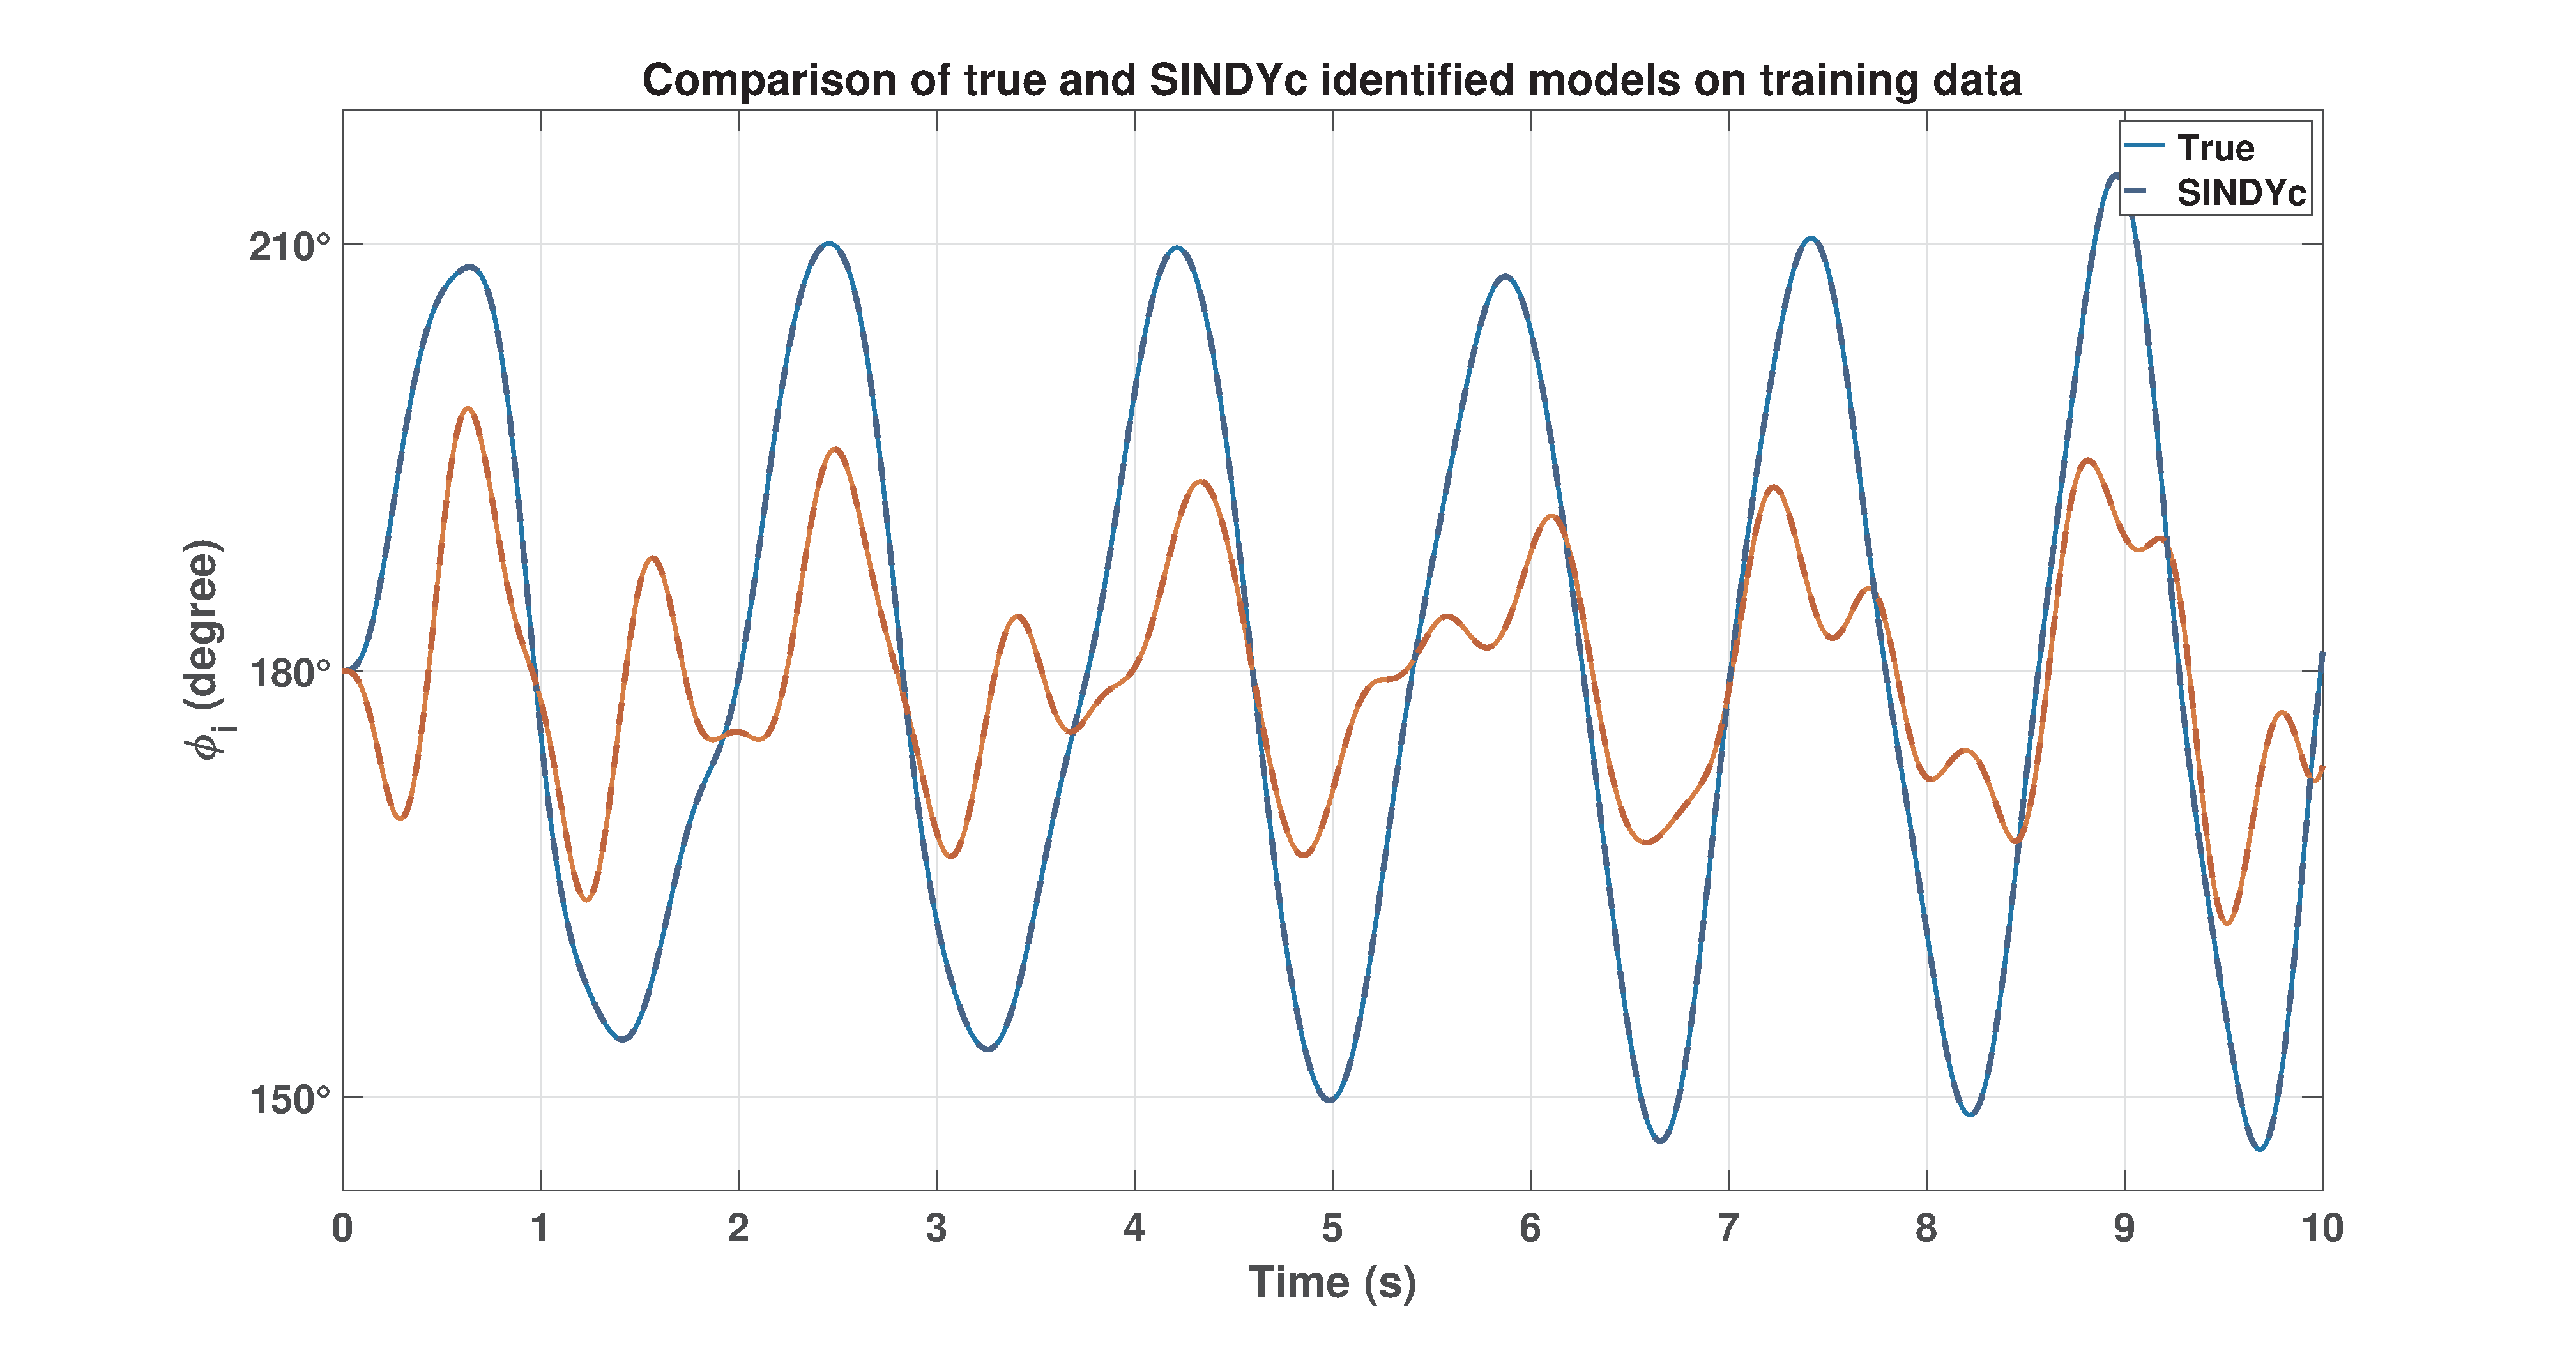
\includegraphics[width=0.915\linewidth]{figures/SingleTrajTrain_2_0_1}
    \caption{Identification with single trajectory and $\mathbf{\Psi_3}$ on training data. (\textcolor{blue}{\textbf{--}}) and (\textcolor{red}{\textbf{--}}) represent the trajectories of $\phi_1$ and $\phi_2$, respectively}
\label{fig:SingleTrajTrain}
\end{figure}
\vspace{0em}
\begin{figure}[ht]
    \centering
    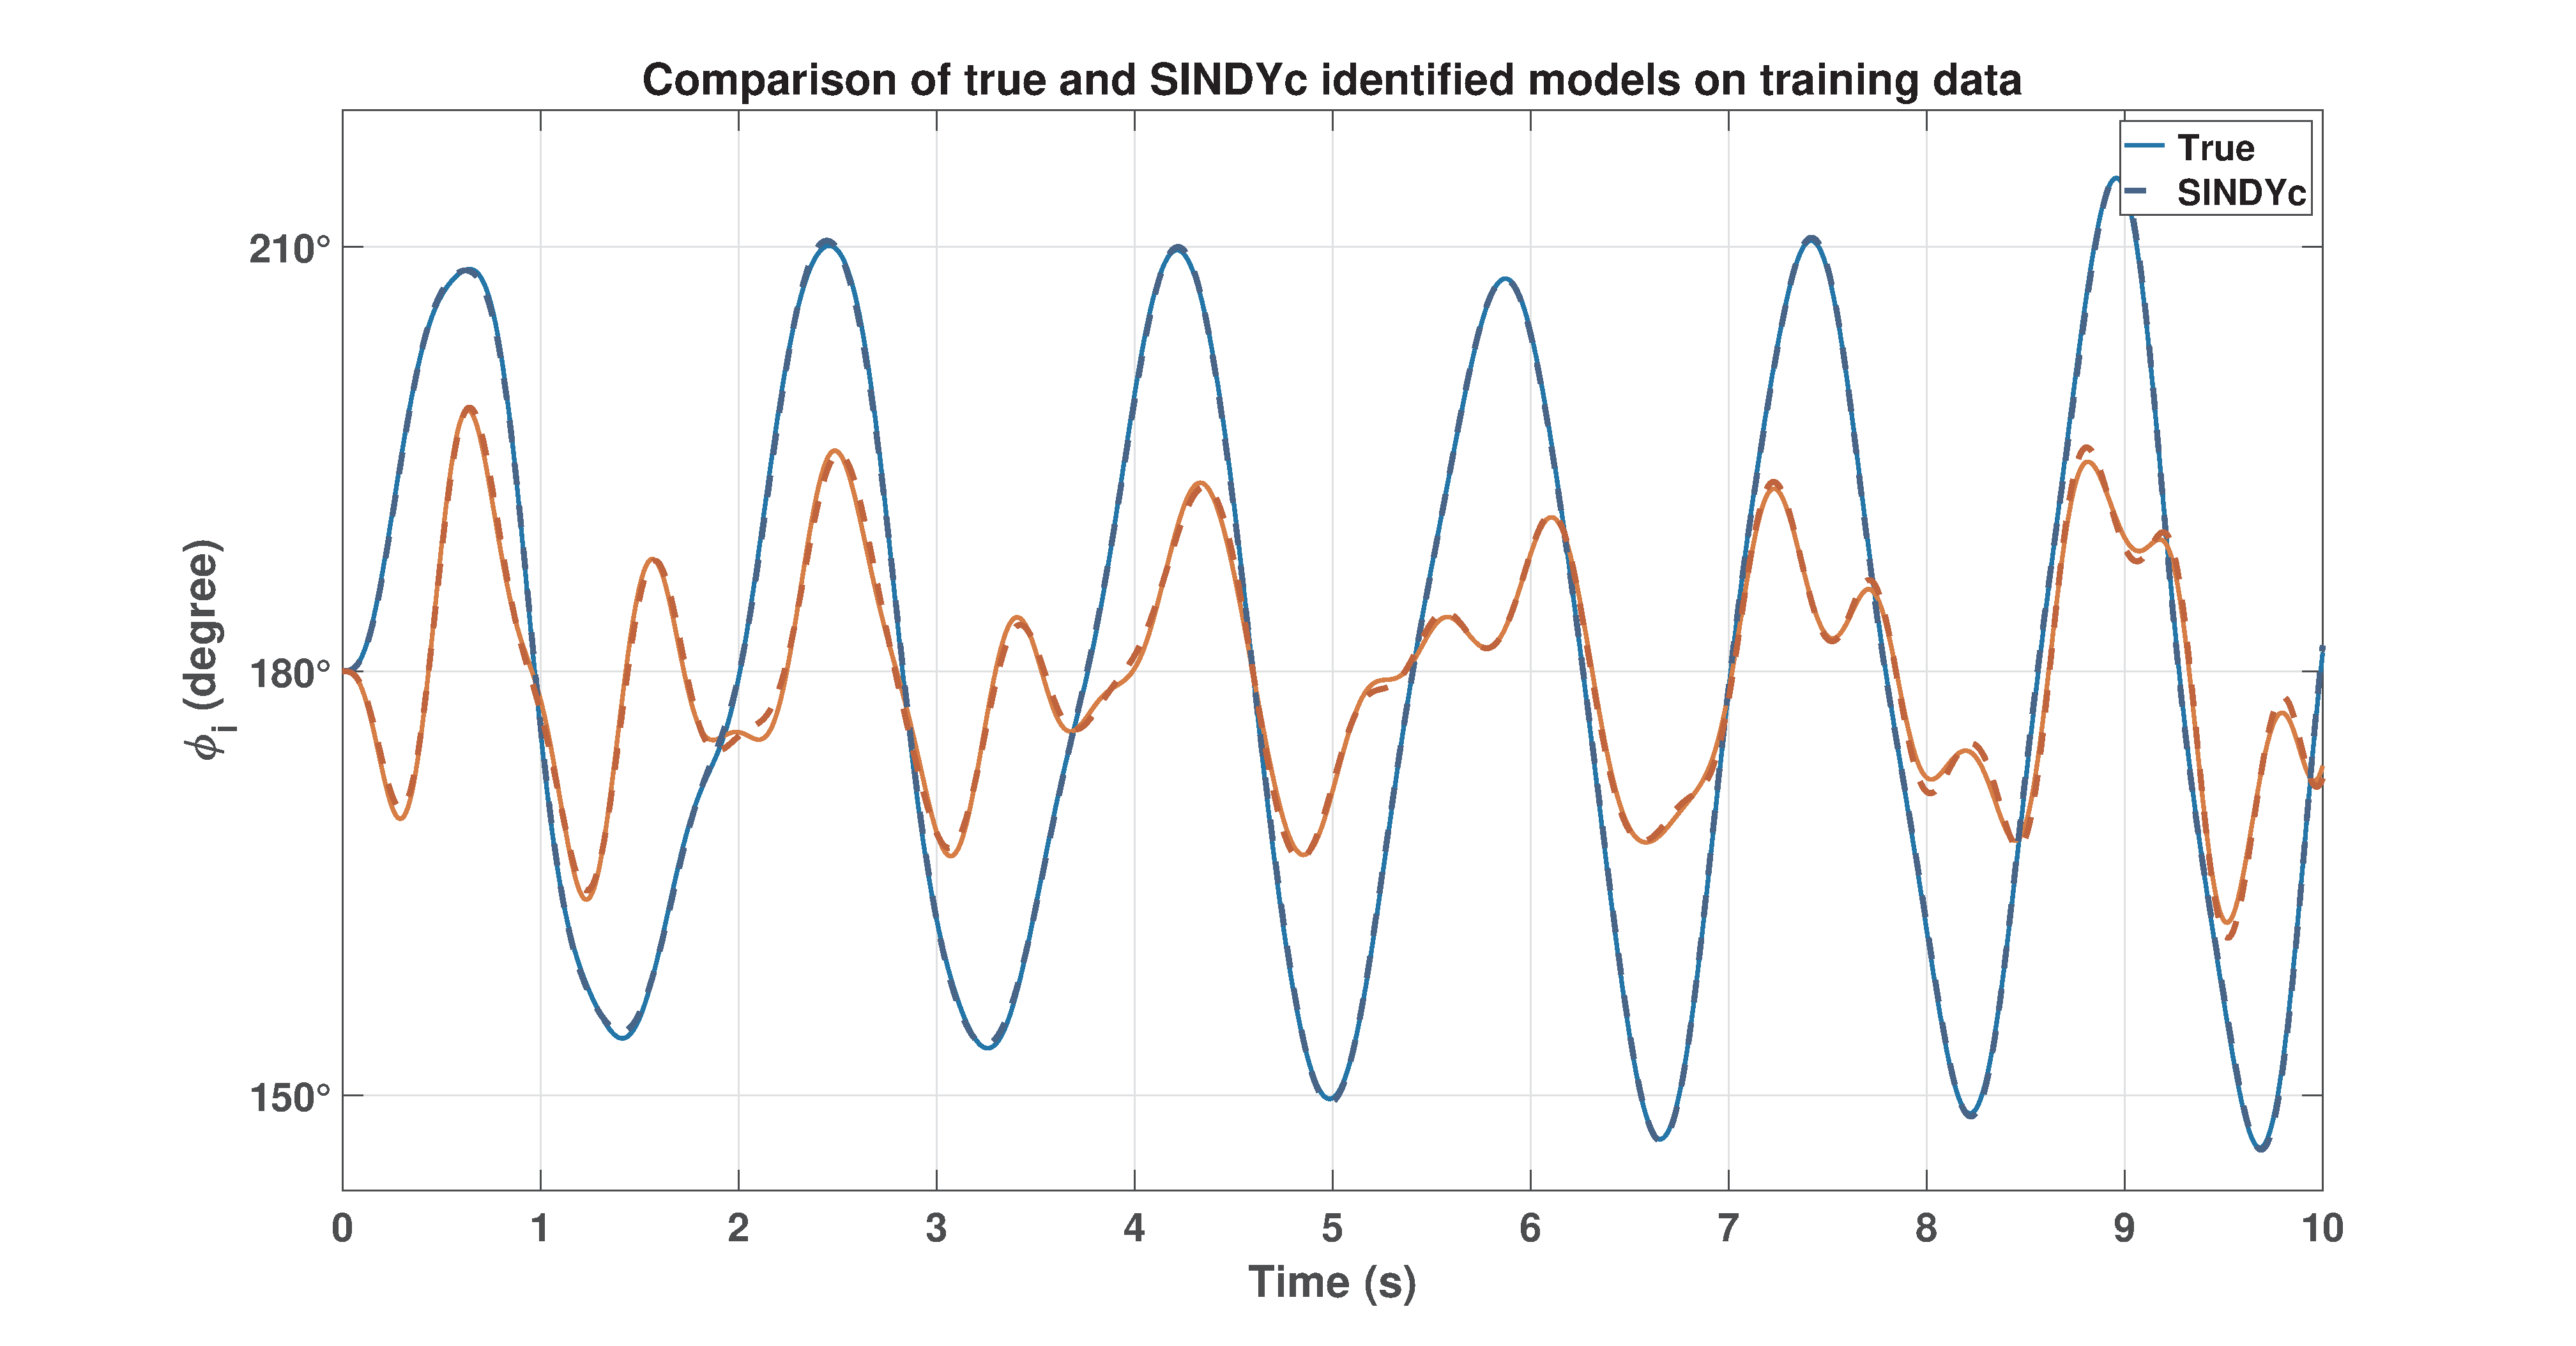
\includegraphics[width=0.915\linewidth]{figures/MultTrajtrain_2_0_1}
    \caption{Identification with multiple trajectories and $\mathbf{\Psi_3}$ on training data.}
    \label{fig: MultTrajTrain}
\end{figure}
% 
% 
\begin{figure}[ht]
    \centering
    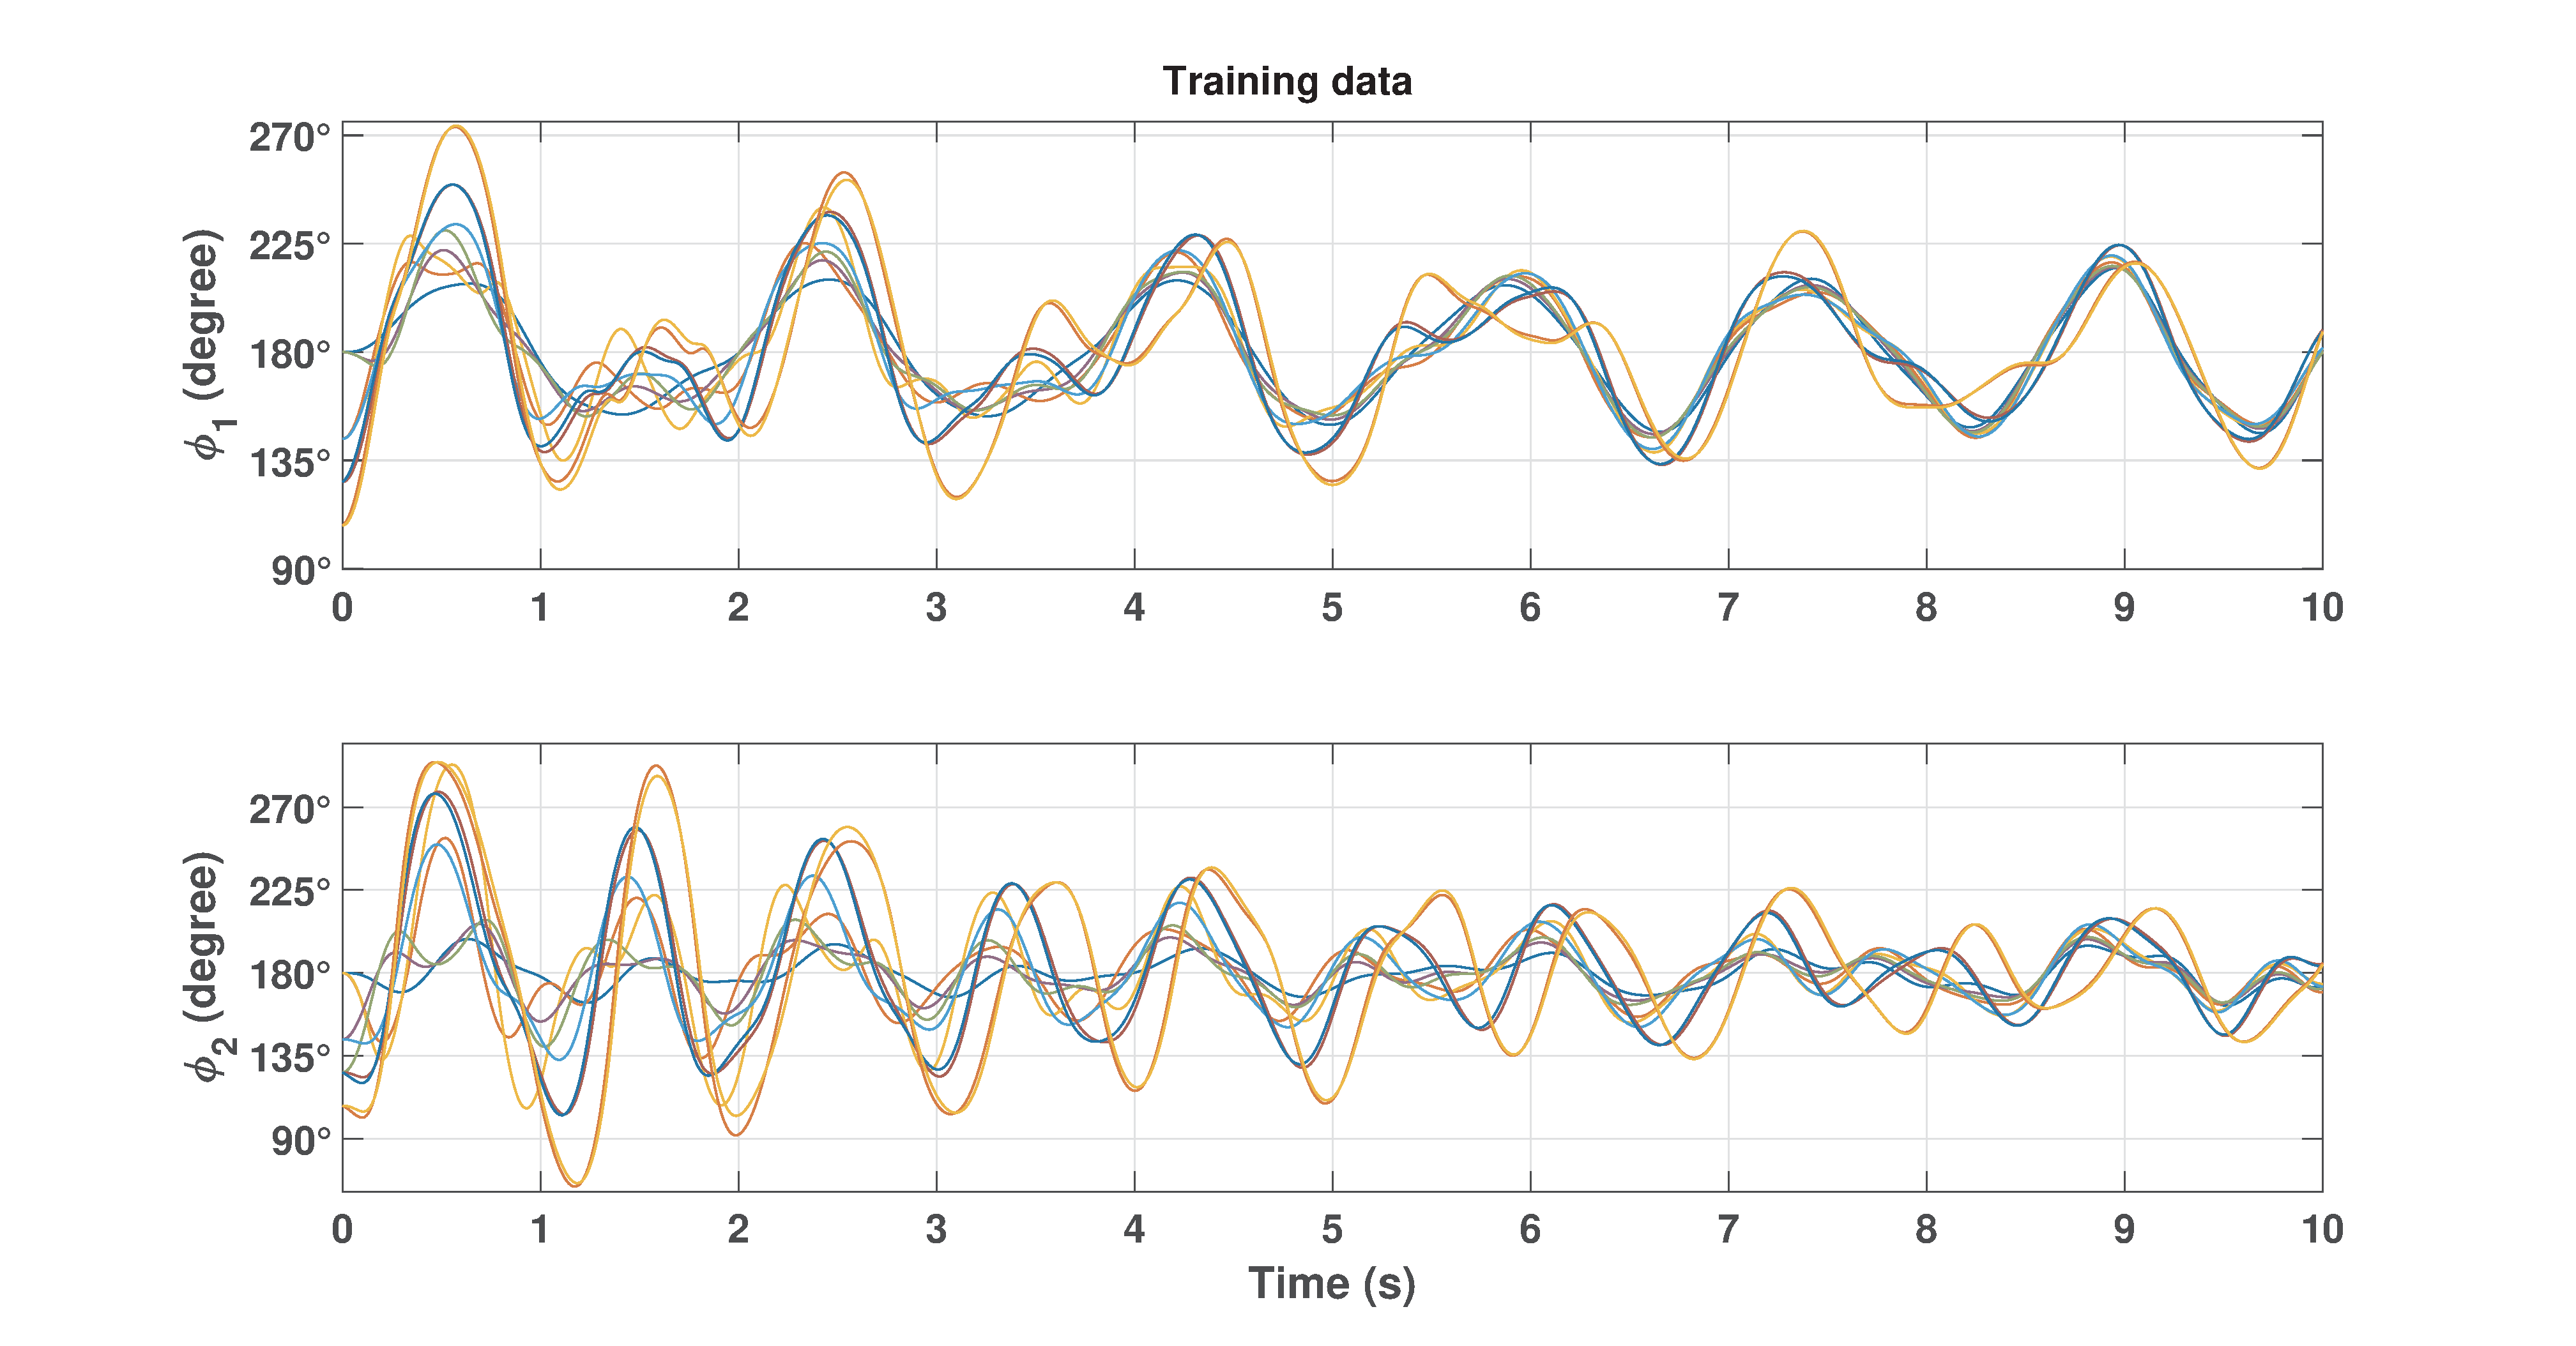
\includegraphics[width=1\linewidth]{figures/TrainingData}
    \caption{Training data from multiple trajectories}
    \label{fig:TrainingData}
\end{figure}
\newpage
In the above figures, $\mathbf{\Psi_3}$ is a vector of observables that is already defined in Section \ref{Chapter:Data}. From the above figures, one can see that the SINDYc algorithm almost perfectly identifies the time evolution of the state trajectories both in the case of training data obtained from a single initial condition and multiple initial conditions for a specific choice of candidate functions.\par
Even though it might seem that data from a single trajectory is enough to approximate the dynamics, this will almost always fail when the system is forced with a forcing function that is different from the forcing function used to generate the training data. Revisiting Section \ref{sec:SINDy}, SINDY-with-control~(SINDYc) computes a (tall) sparse matrix of coefficients of the candidate functions $\mathbf{\Xi}$ (which also contains the input function), and this matrix of coefficients is then used to simulate the dynamics for a new forcing function. Figures \ref{fig:SingleTrajVal} and \ref{fig: MultTrajVal} show the prediction of dynamics evaluated on the matrix of coefficients generated from training data for a new `validation' forcing function in (\ref{Eq:Forcing}). It is interesting to note that while the $\mathbf{\Xi}$ generated from a single trajectory worked perfectly well for data that lies within the range of training data, it fails to correlate the dynamics over a longer time span when the forcing function drives the trajectory away from the training trajectory, as observed in Fig \ref{fig:SingleTrajVal}. The predicted trajectory by SINDYc fails to follow the reference trajectory after approximately 1.5 seconds, where both the amplitude and the frequency of the reference trajectory differ from the trajectory used for training. Whereas, in Fig.~\ref{fig: MultTrajVal} it is seen that the dynamics are approximately predicted for $\mathbf{\Xi}$ generated from multiple trajectories for a `good' choice of observables. Therefore, it is vital to generate data from multiple trajectories and train the regressors, be it SINDYc or EDMDc, for a close approximation of the dynamics. 
% 
\begin{figure}[ht]
    \centering
    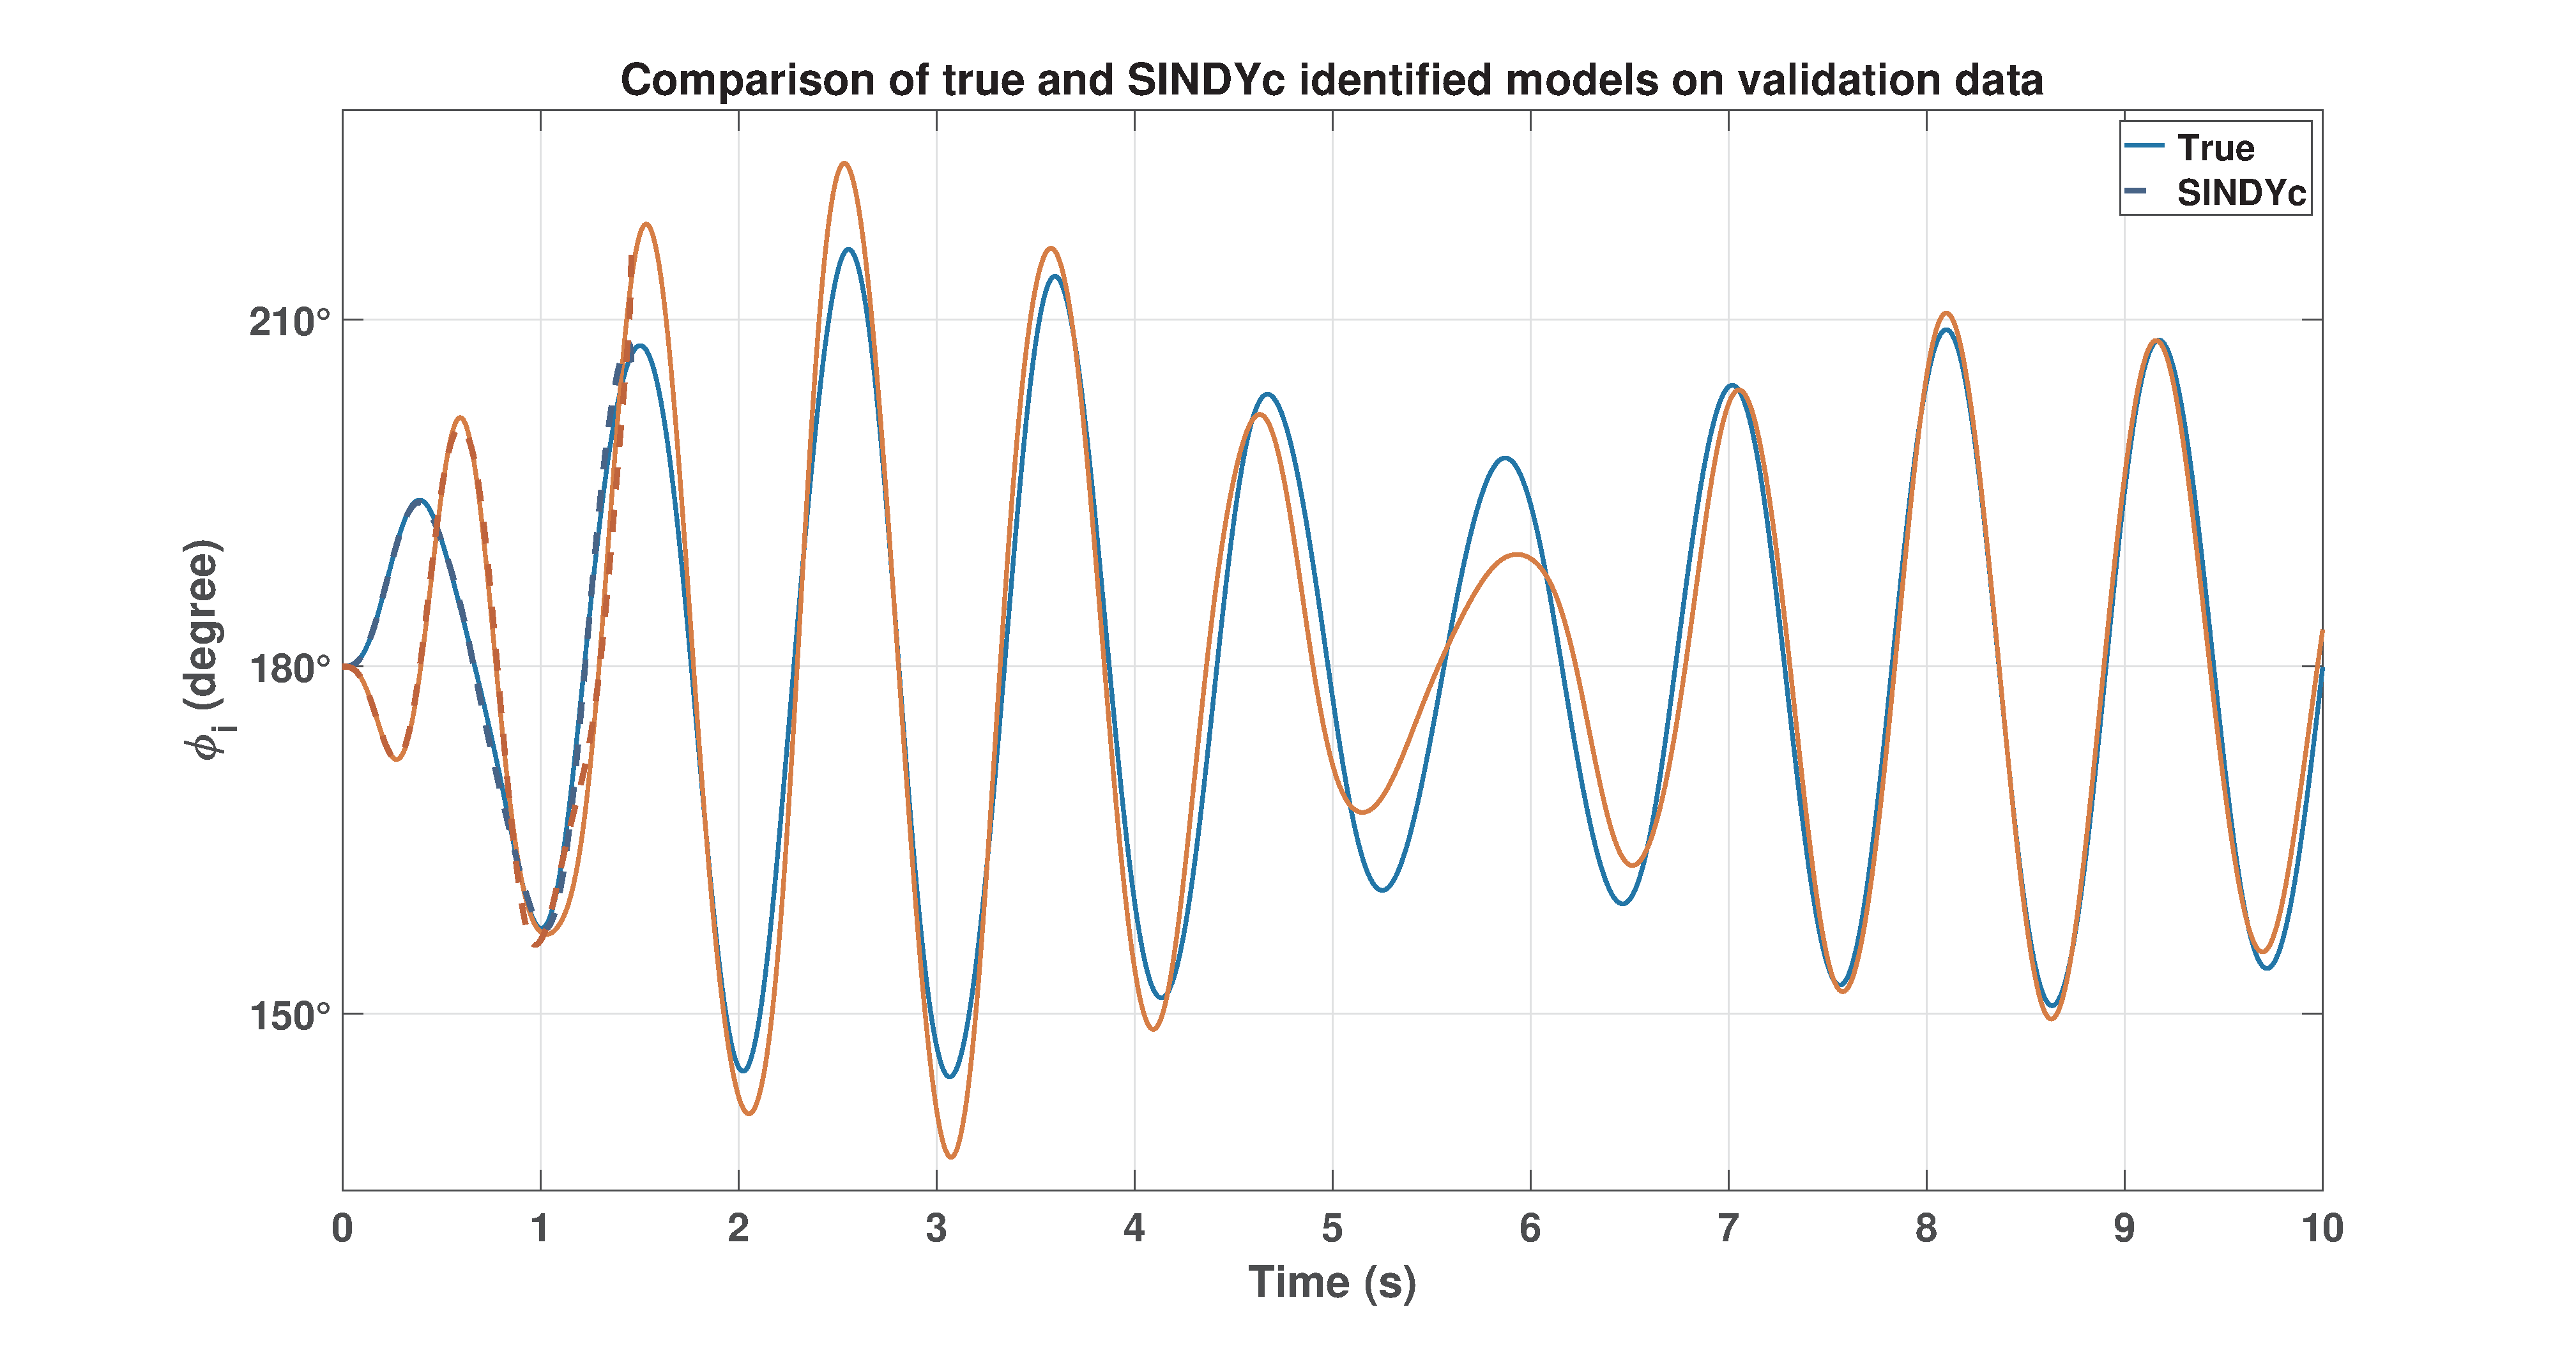
\includegraphics[width=1\linewidth]{figures/SingleTrajVal_2_0_1}
    \caption{Identification with single trajectory and $\mathbf{\Psi_3}$ on validation data}
    \label{fig:SingleTrajVal}
\end{figure}
% 
\begin{figure}[ht]
    \centering
    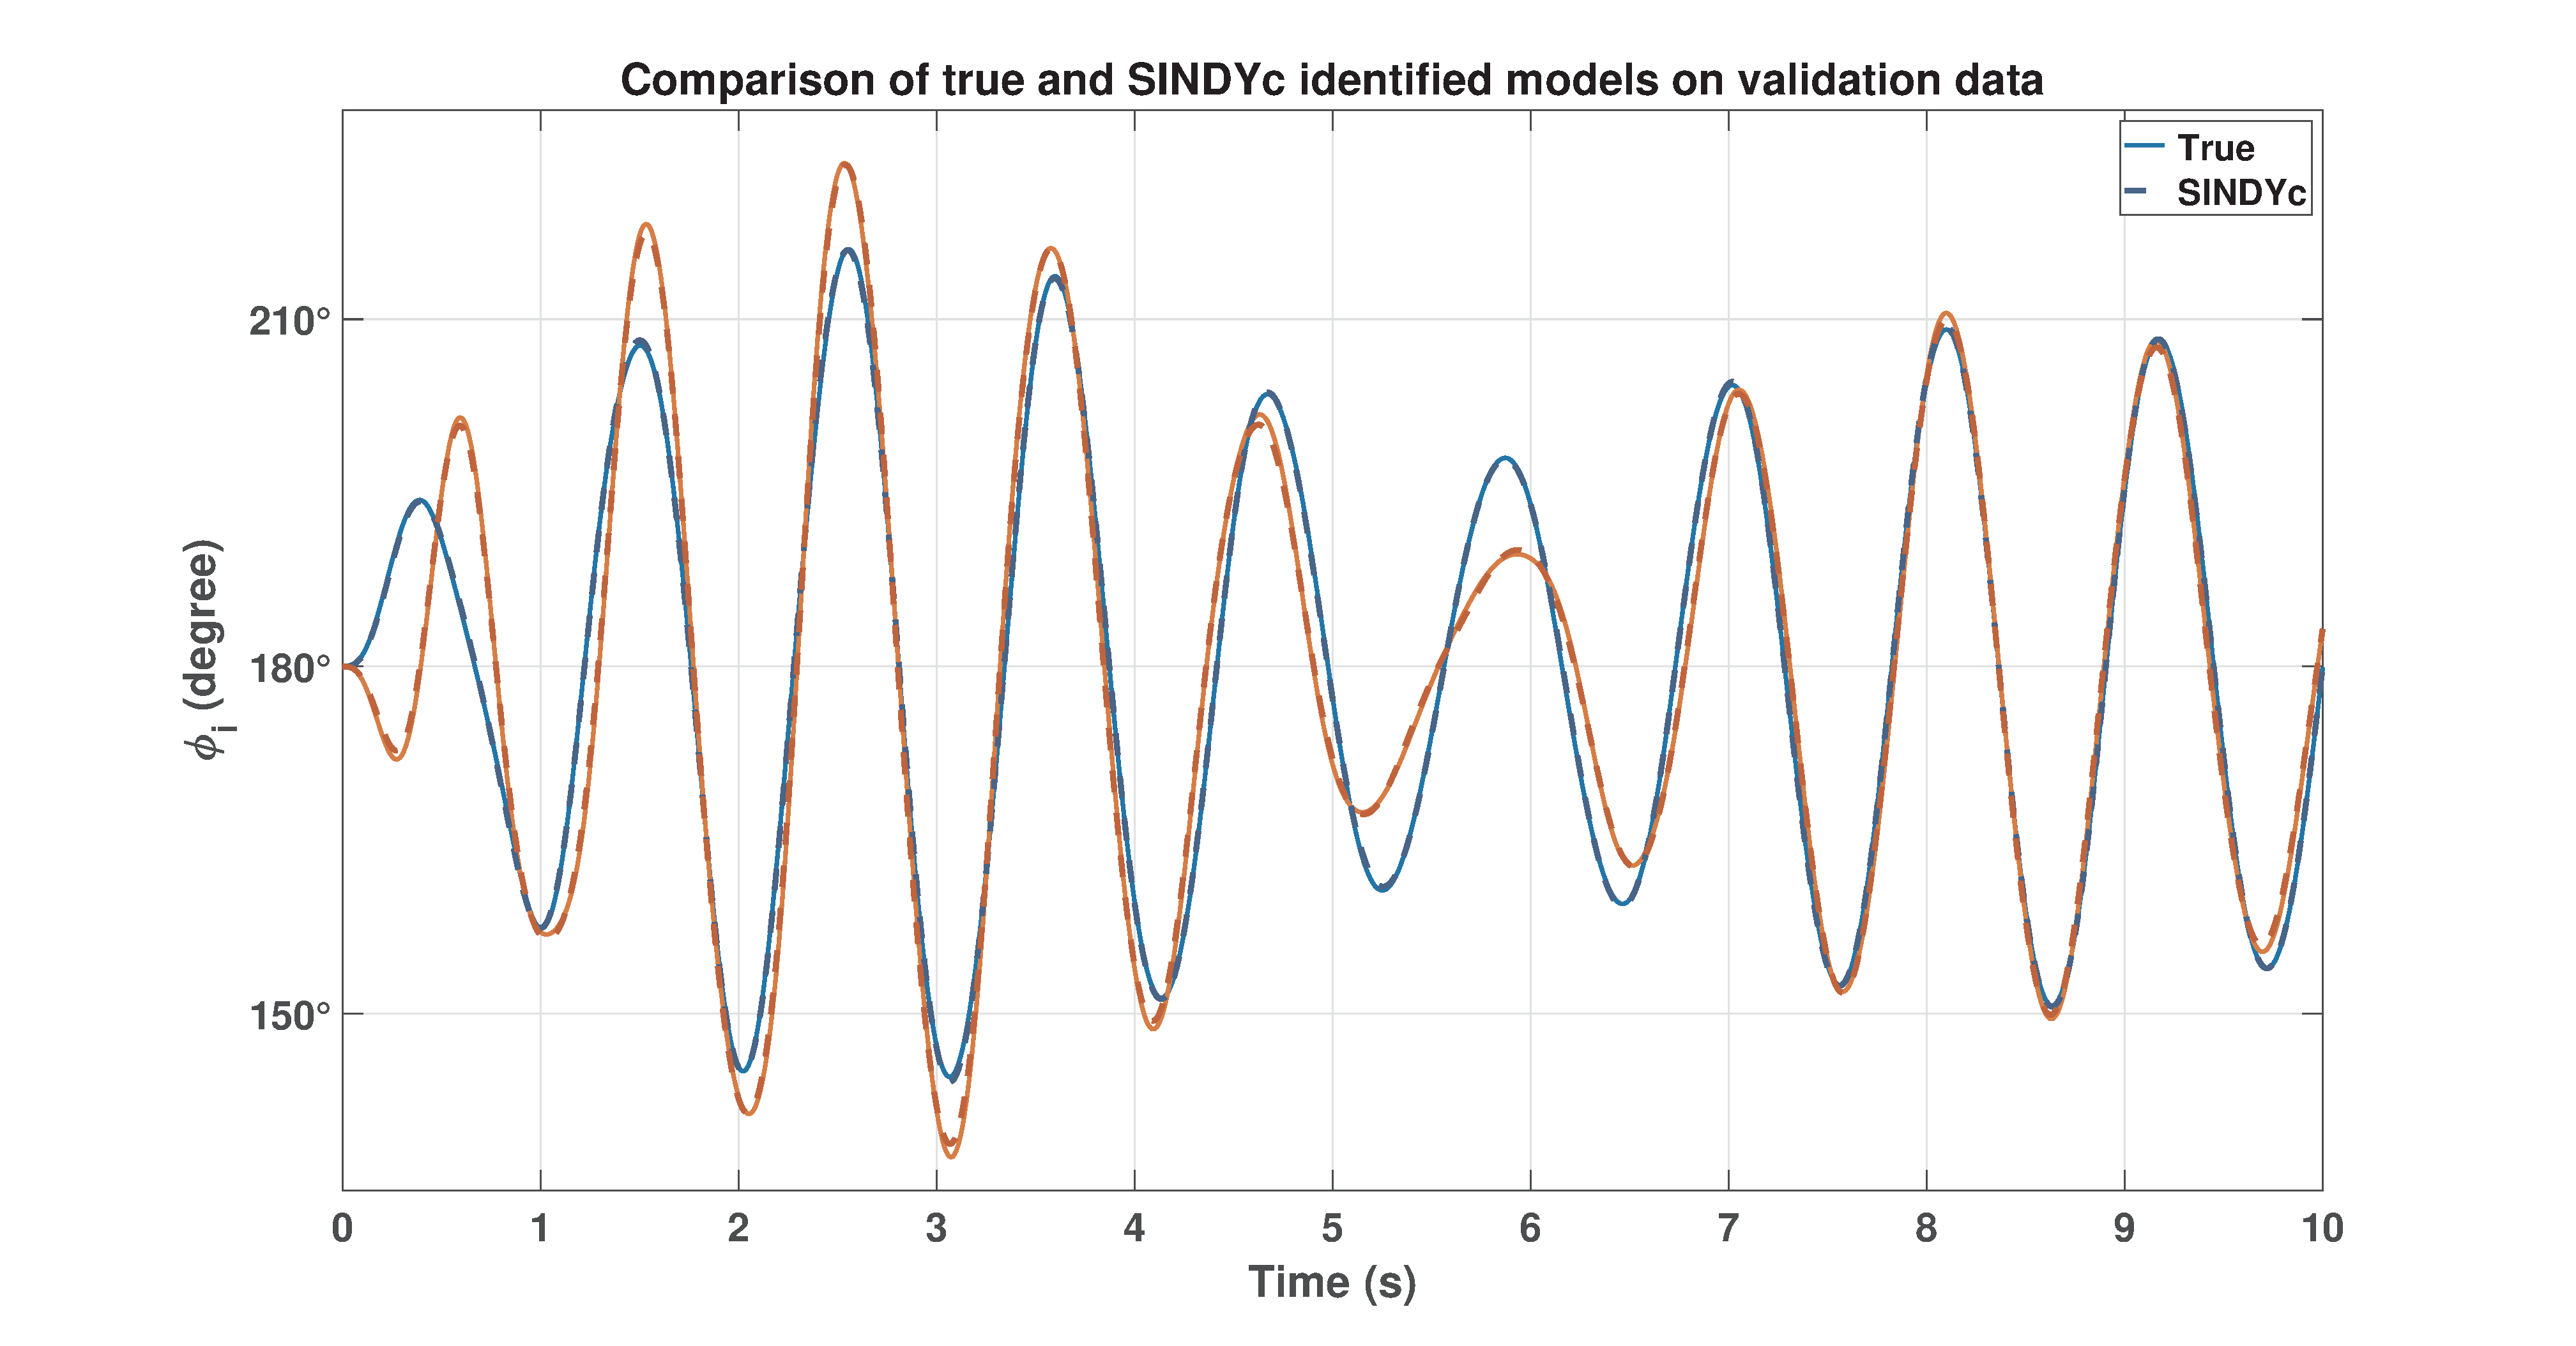
\includegraphics[width=1\linewidth]{figures/MultTrajVal_2_0_1}
    \caption{Identification with multiple trajectories and $\mathbf{\Psi_3}$ on validation data}
    \label{fig: MultTrajVal}
\end{figure}
% 
\newpage
Figures \ref{fig: inputTrainVal}, \ref{fig: SingleTrajValCombo} and \ref{fig: MultTrajValCombo} visualize forcing functions and the consequent predictions with a slightly different forcing function from earlier but still within the range defined by (\ref{Eq:Forcing}). The forcing function used here for training is a chirp signal with a constant frequency. Again, it is seen that model approximated from data generated by multiple trajectories performs better.
\begin{figure}[H]
    \centering
    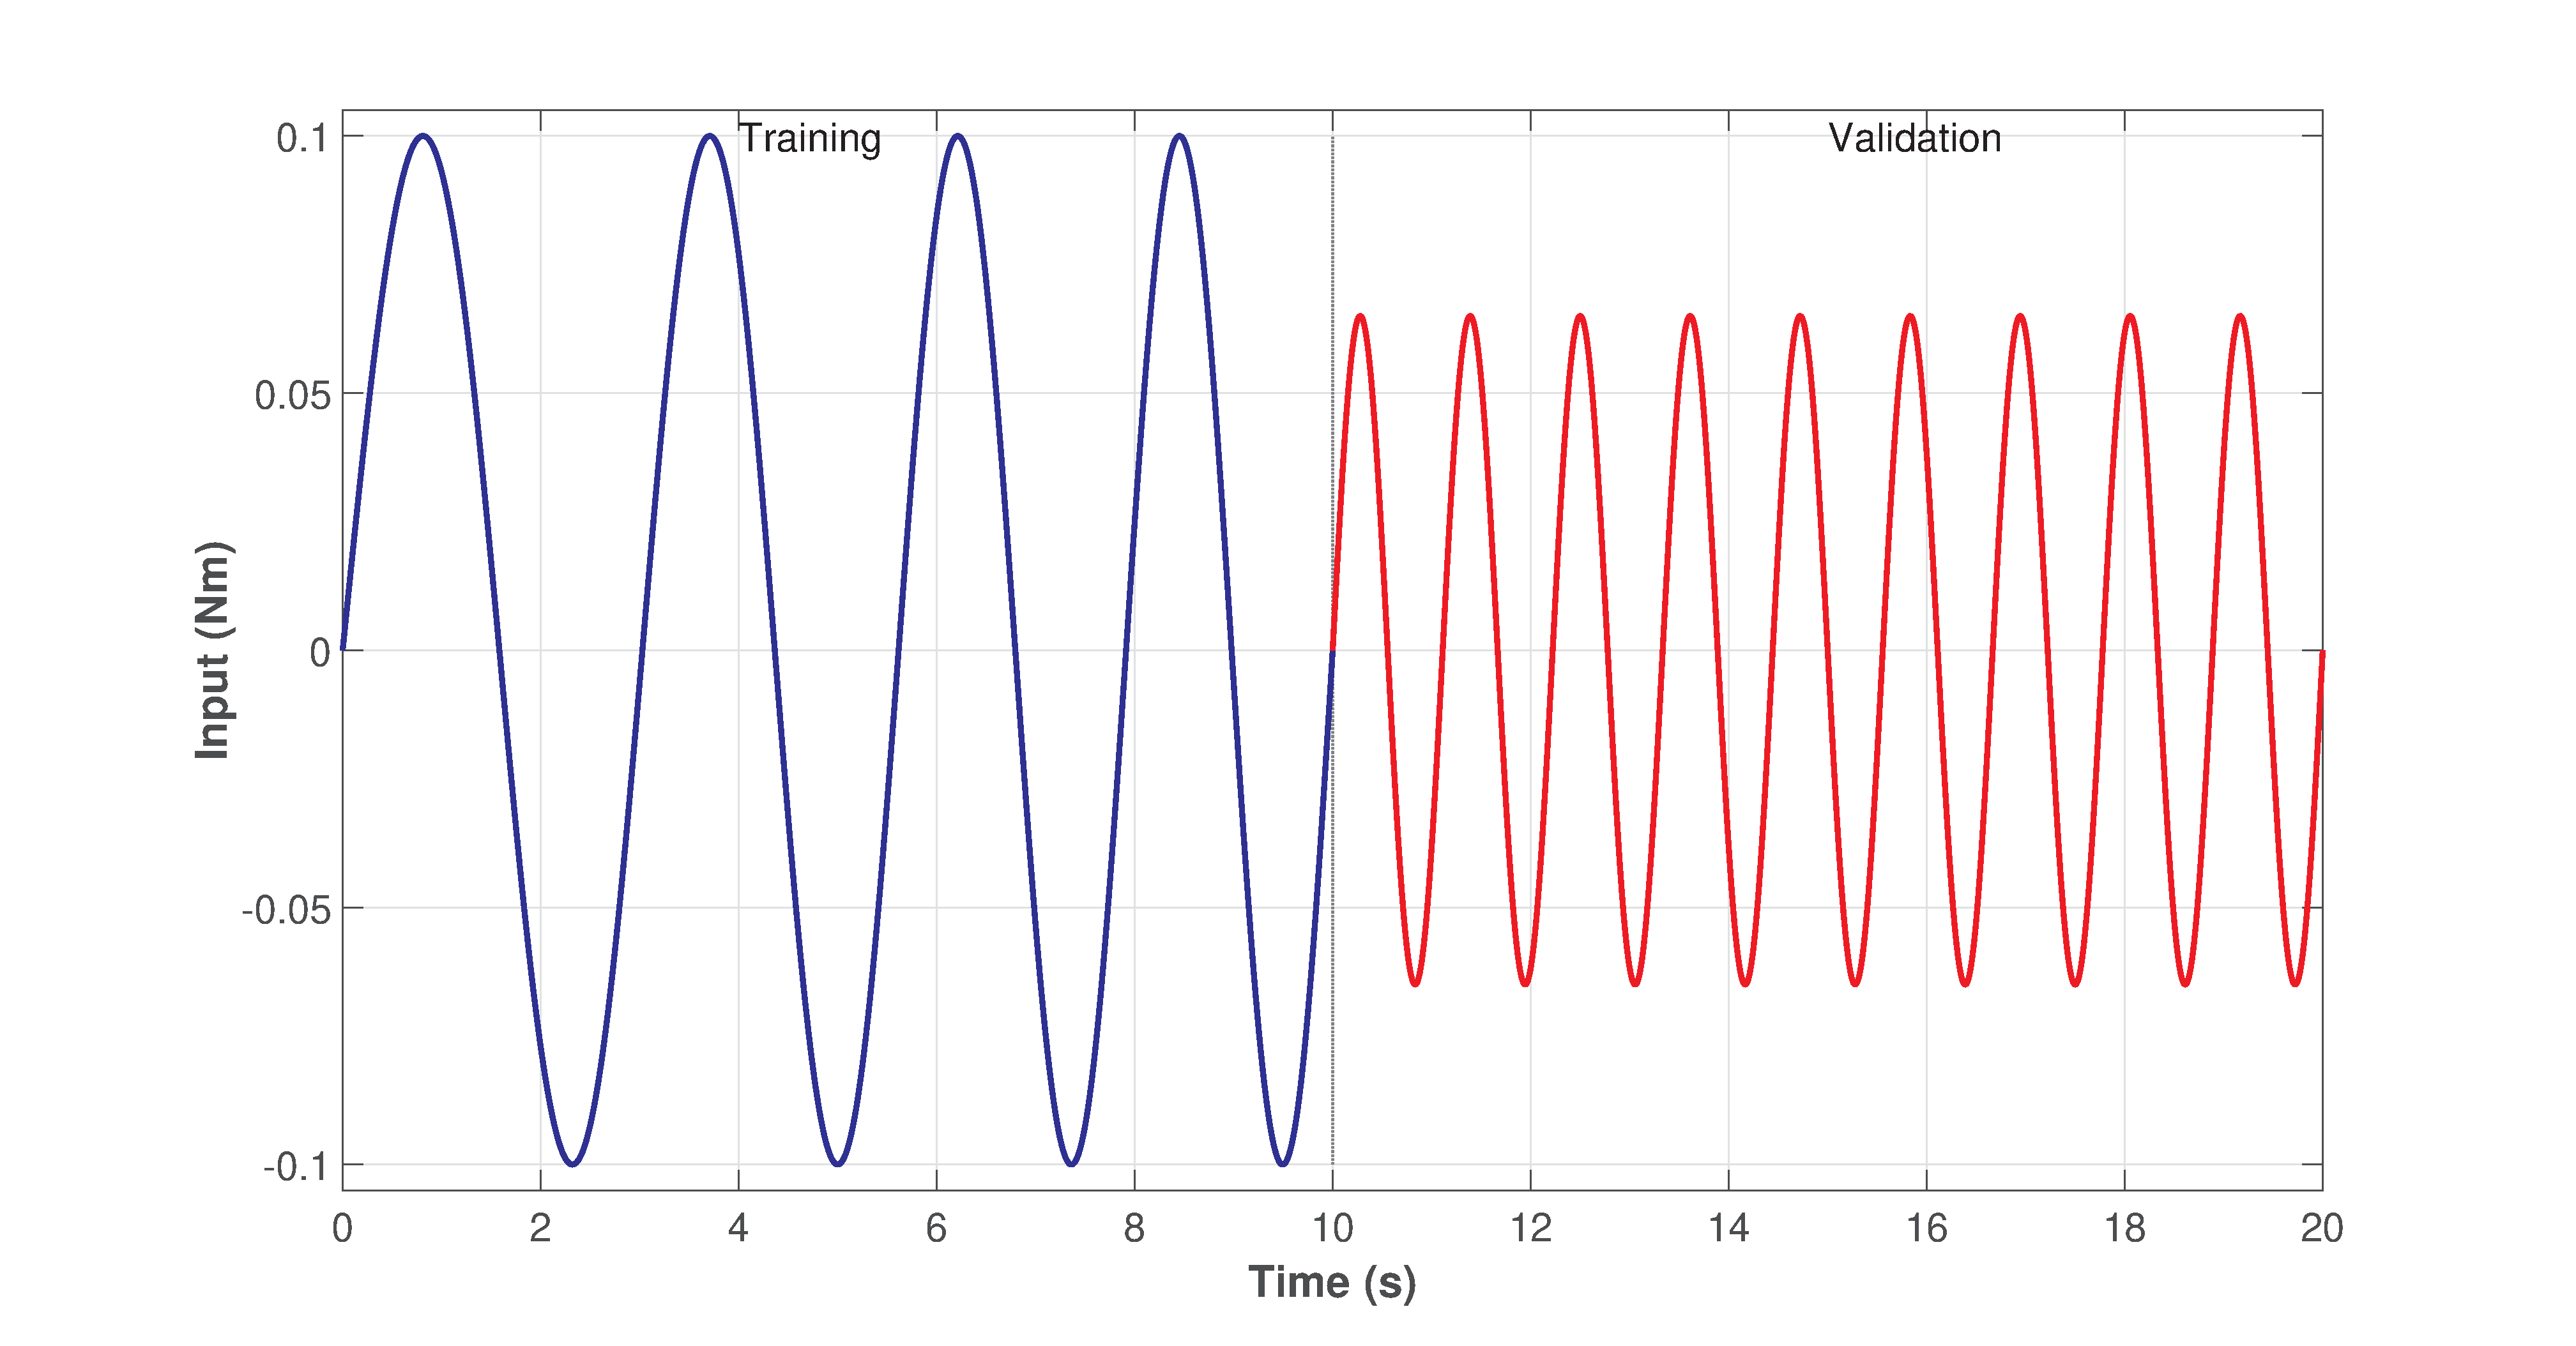
\includegraphics[width=0.85\linewidth]{figures/Input}
    \caption{The training and validation inputs}
    \label{fig: inputTrainVal}
% \end{figure}
\vspace{0.005em}
% \begin{figure}[ht]
    \centering
    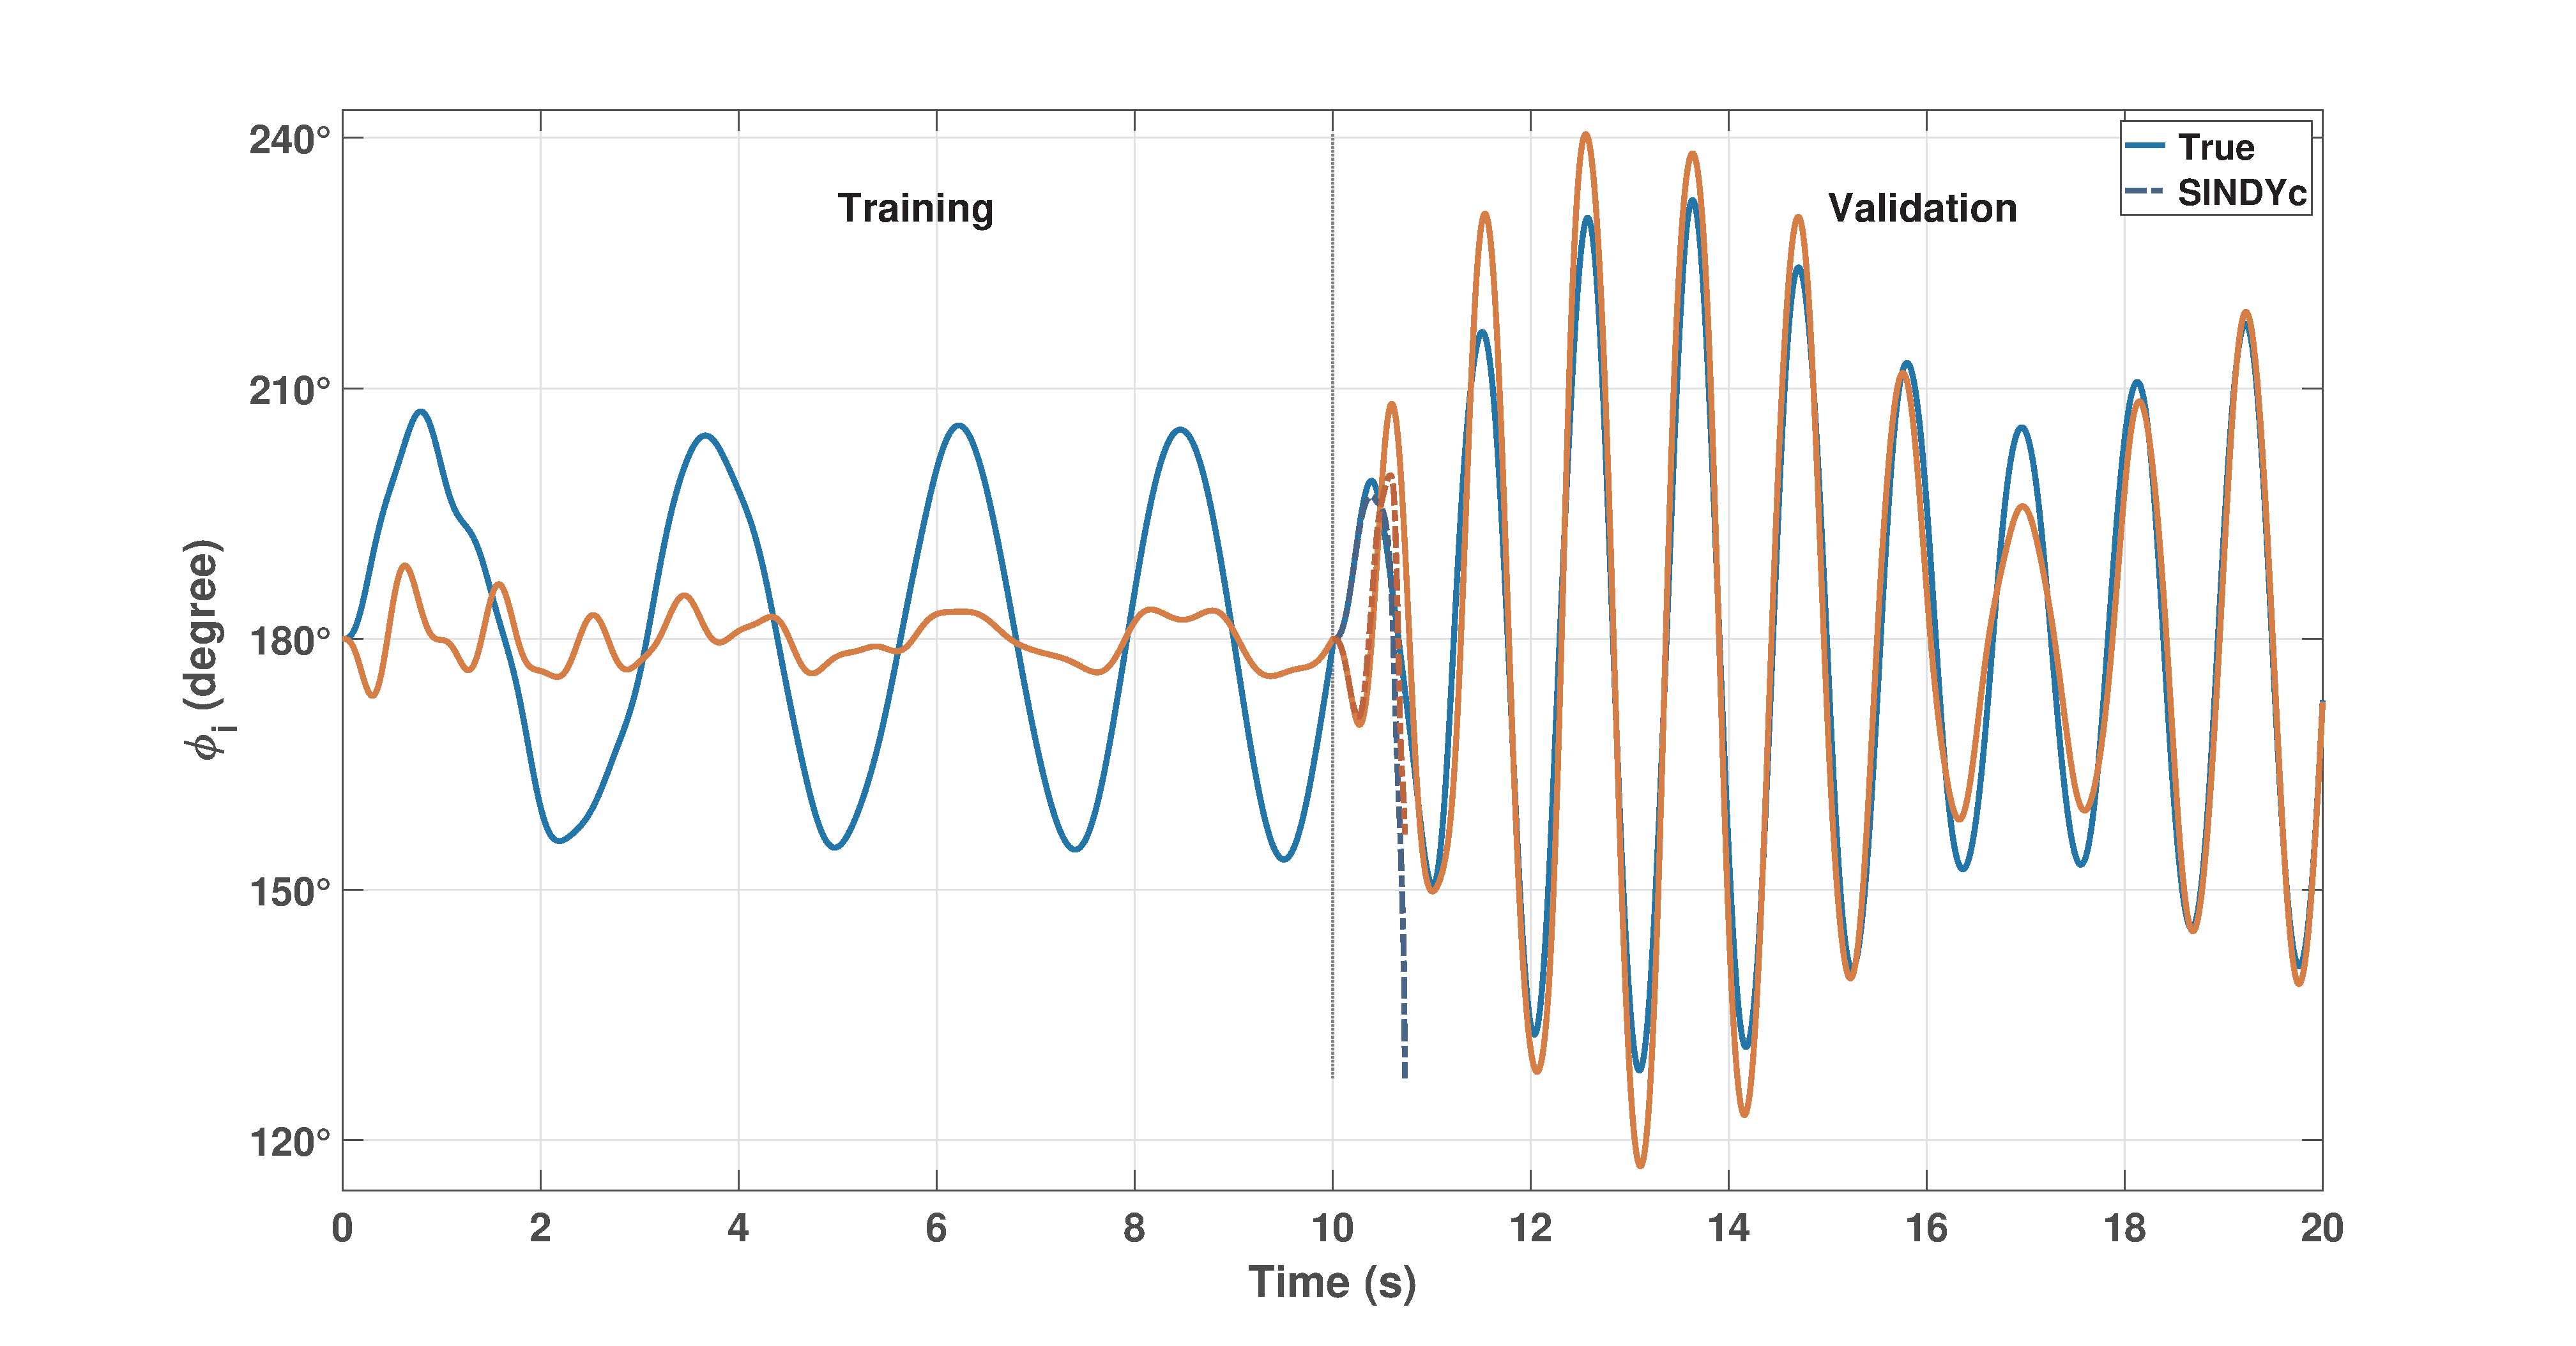
\includegraphics[width=0.85\linewidth]{figures/VizSingleTrajVal_2_0_1}
    \caption{Visualization of the validation with single trajectory and $\mathbf{\Psi_3}$}
    \label{fig: SingleTrajValCombo}
% \end{figure}
\vspace{0.005em}
% \begin{figure}[ht]
    \centering
    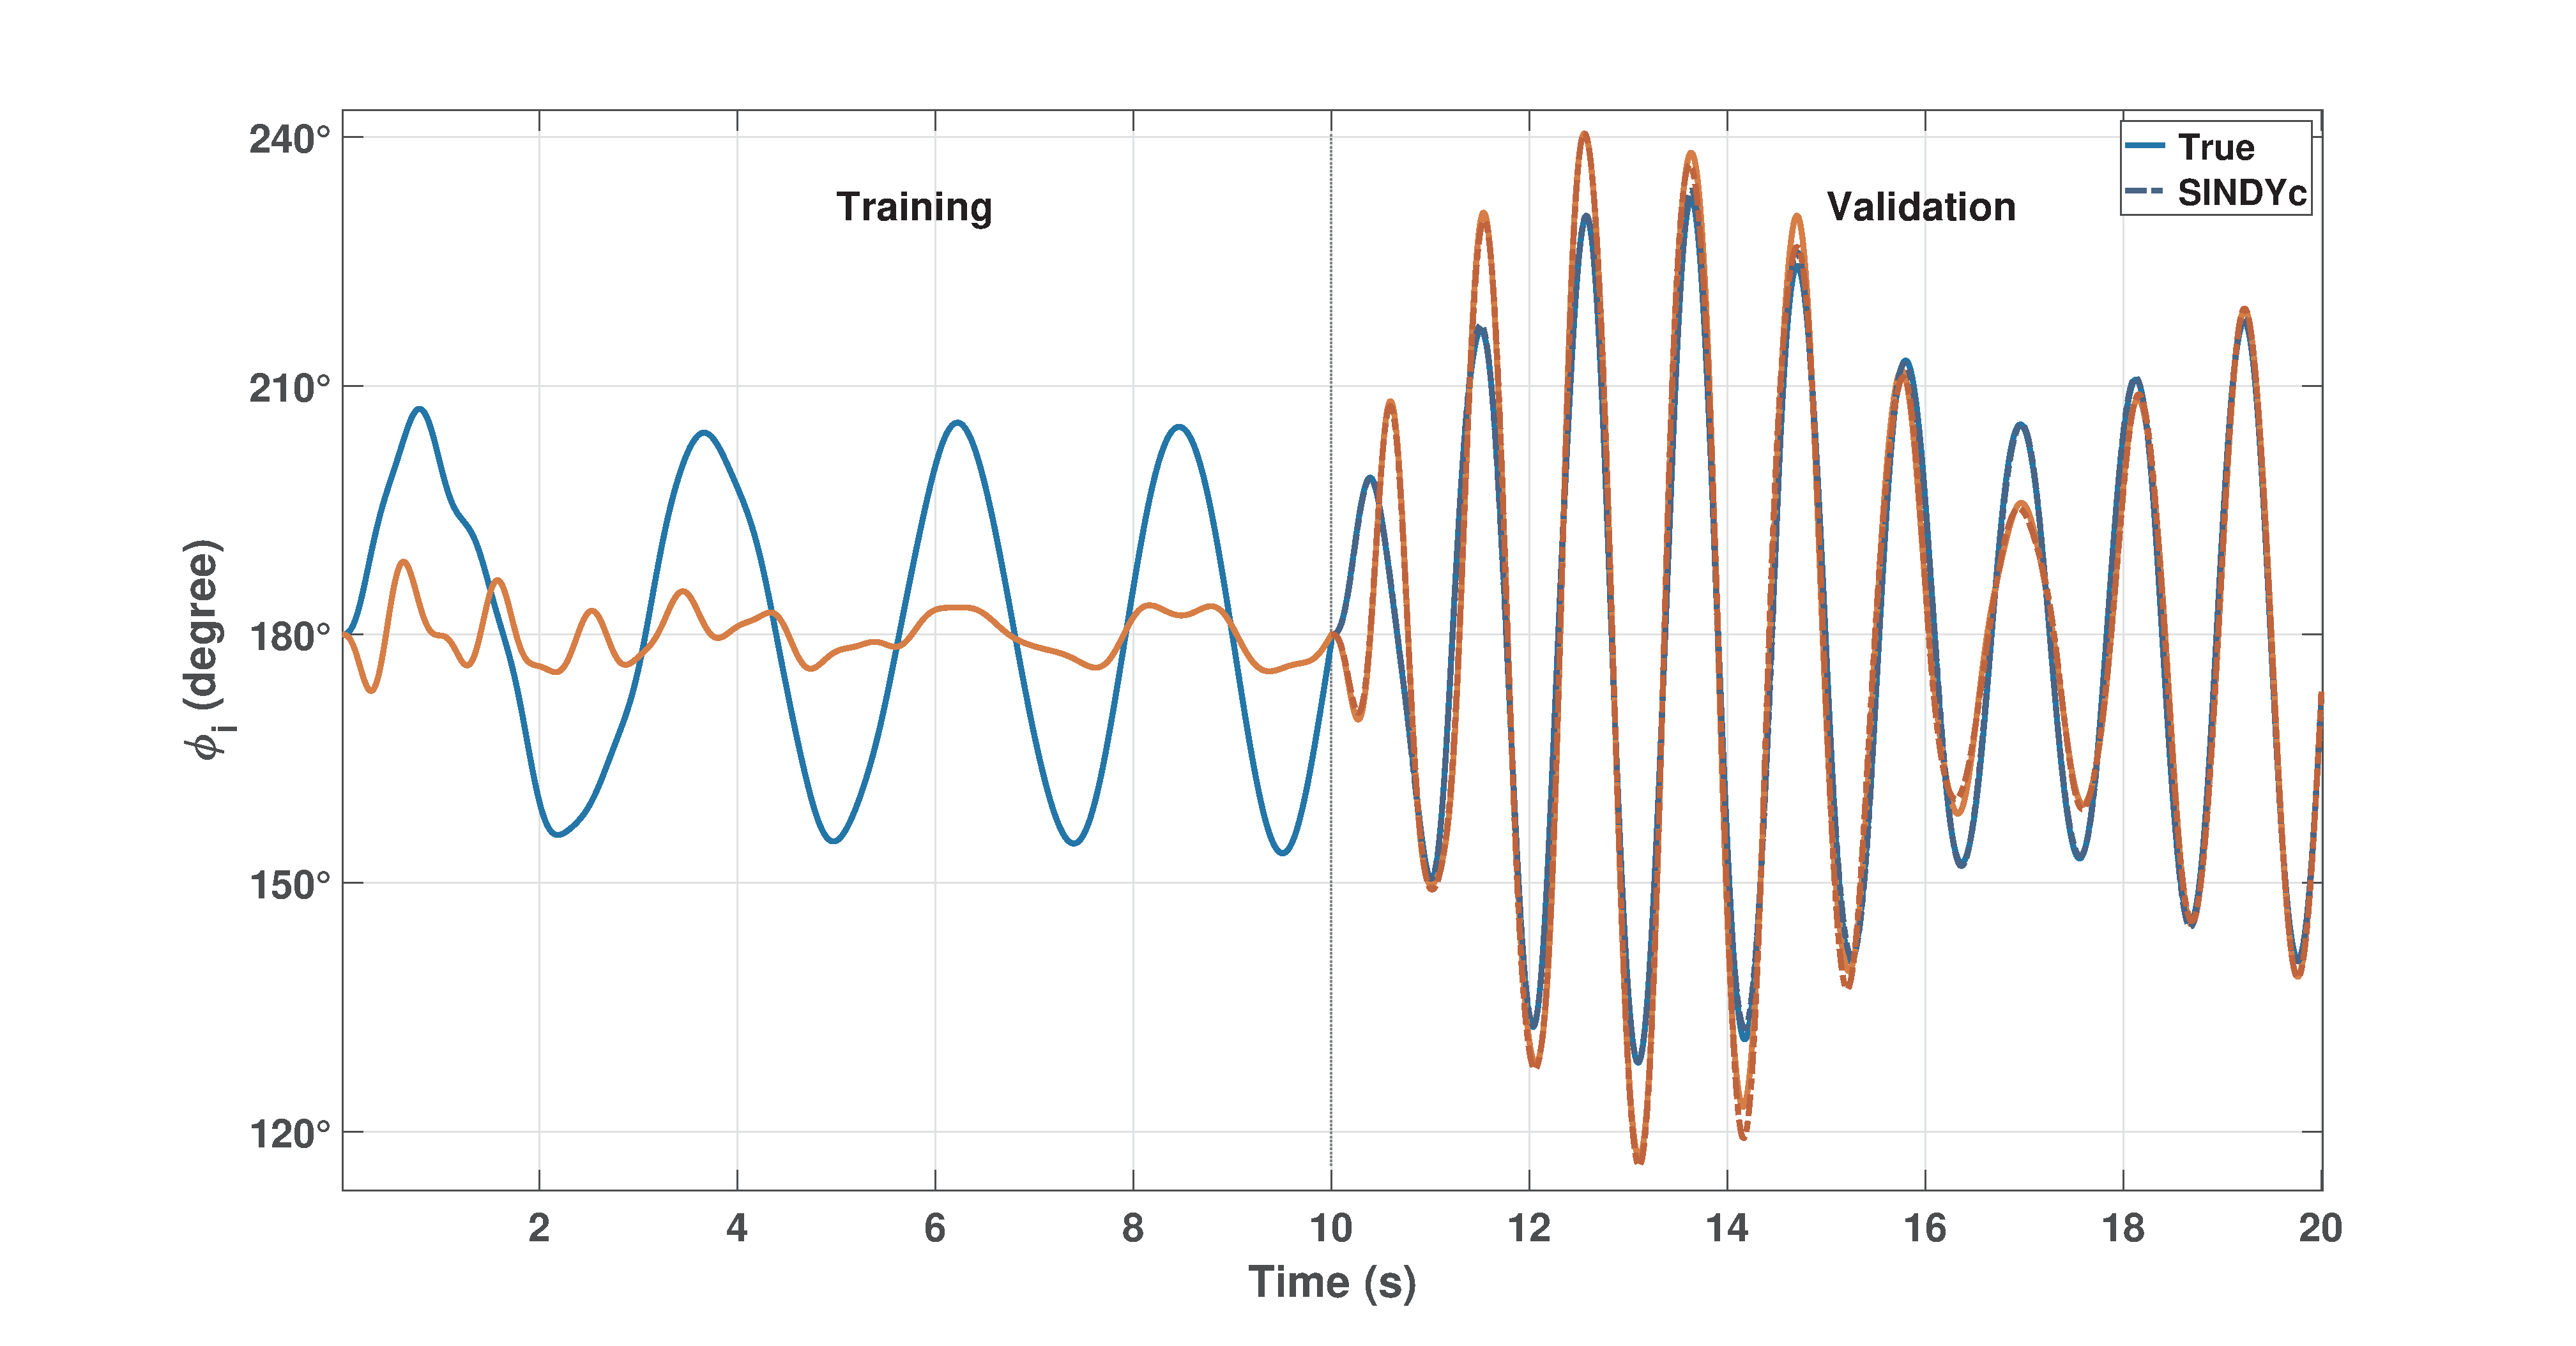
\includegraphics[width=0.85\linewidth]{figures/VizMultTrajVal_2_0_1}
    \caption{Visualization of the validation with multiple trajectories and $\mathbf{\Psi_3}$}
    \label{fig: MultTrajValCombo}
\end{figure}
% 
\newpage
The predictions fit the true trajectories for a specific choice of candidate functions, $\mathbf{\Psi}_3$, in the above figures. Some or all of the linear or nonlinear functions in this set of candidate functions may form the set of observables required to compute the Koopman operator, generating a linear approximation of the underlying nonlinear system. The sparse coefficients matrix $\mathbf{\Xi}$ is a good indicator of such dominant linear or nonlinear functions which can then be considered as observables. It is important to note that the choice of candidate functions, and consequently, the choice of observables is highly subjective, and there are no fixed rules/methods to choose them. Some of the ways have been discussed in Chapter \ref{Chapter:Intro}. Figure \ref{fig: MultTrajVal2} illustrates the effect of choice of candidate functions. The set of candidate functions used in this case to generate the $\mathbf{\Xi} $ is $\mathbf{\Psi}_2$ which is a set of polynomials up to a second degree. It is seen that $\mathbf{\Psi_2}$ can only approximate the dynamics in a small region around the stable equilibrium after which the predicted trajectories do not behave like the reference trajectory. On the other hand, in Figure \ref{fig: MultTrajVal}, the predicted trajectories closely match the true trajectory. This shows that as one moves away from the desired equilibrium point, the initial state vector needs to be augmented with other nonlinear functions to enable predictions over longer time spans and/or over a larger range.
% 
\begin{figure}[H]
    \centering
    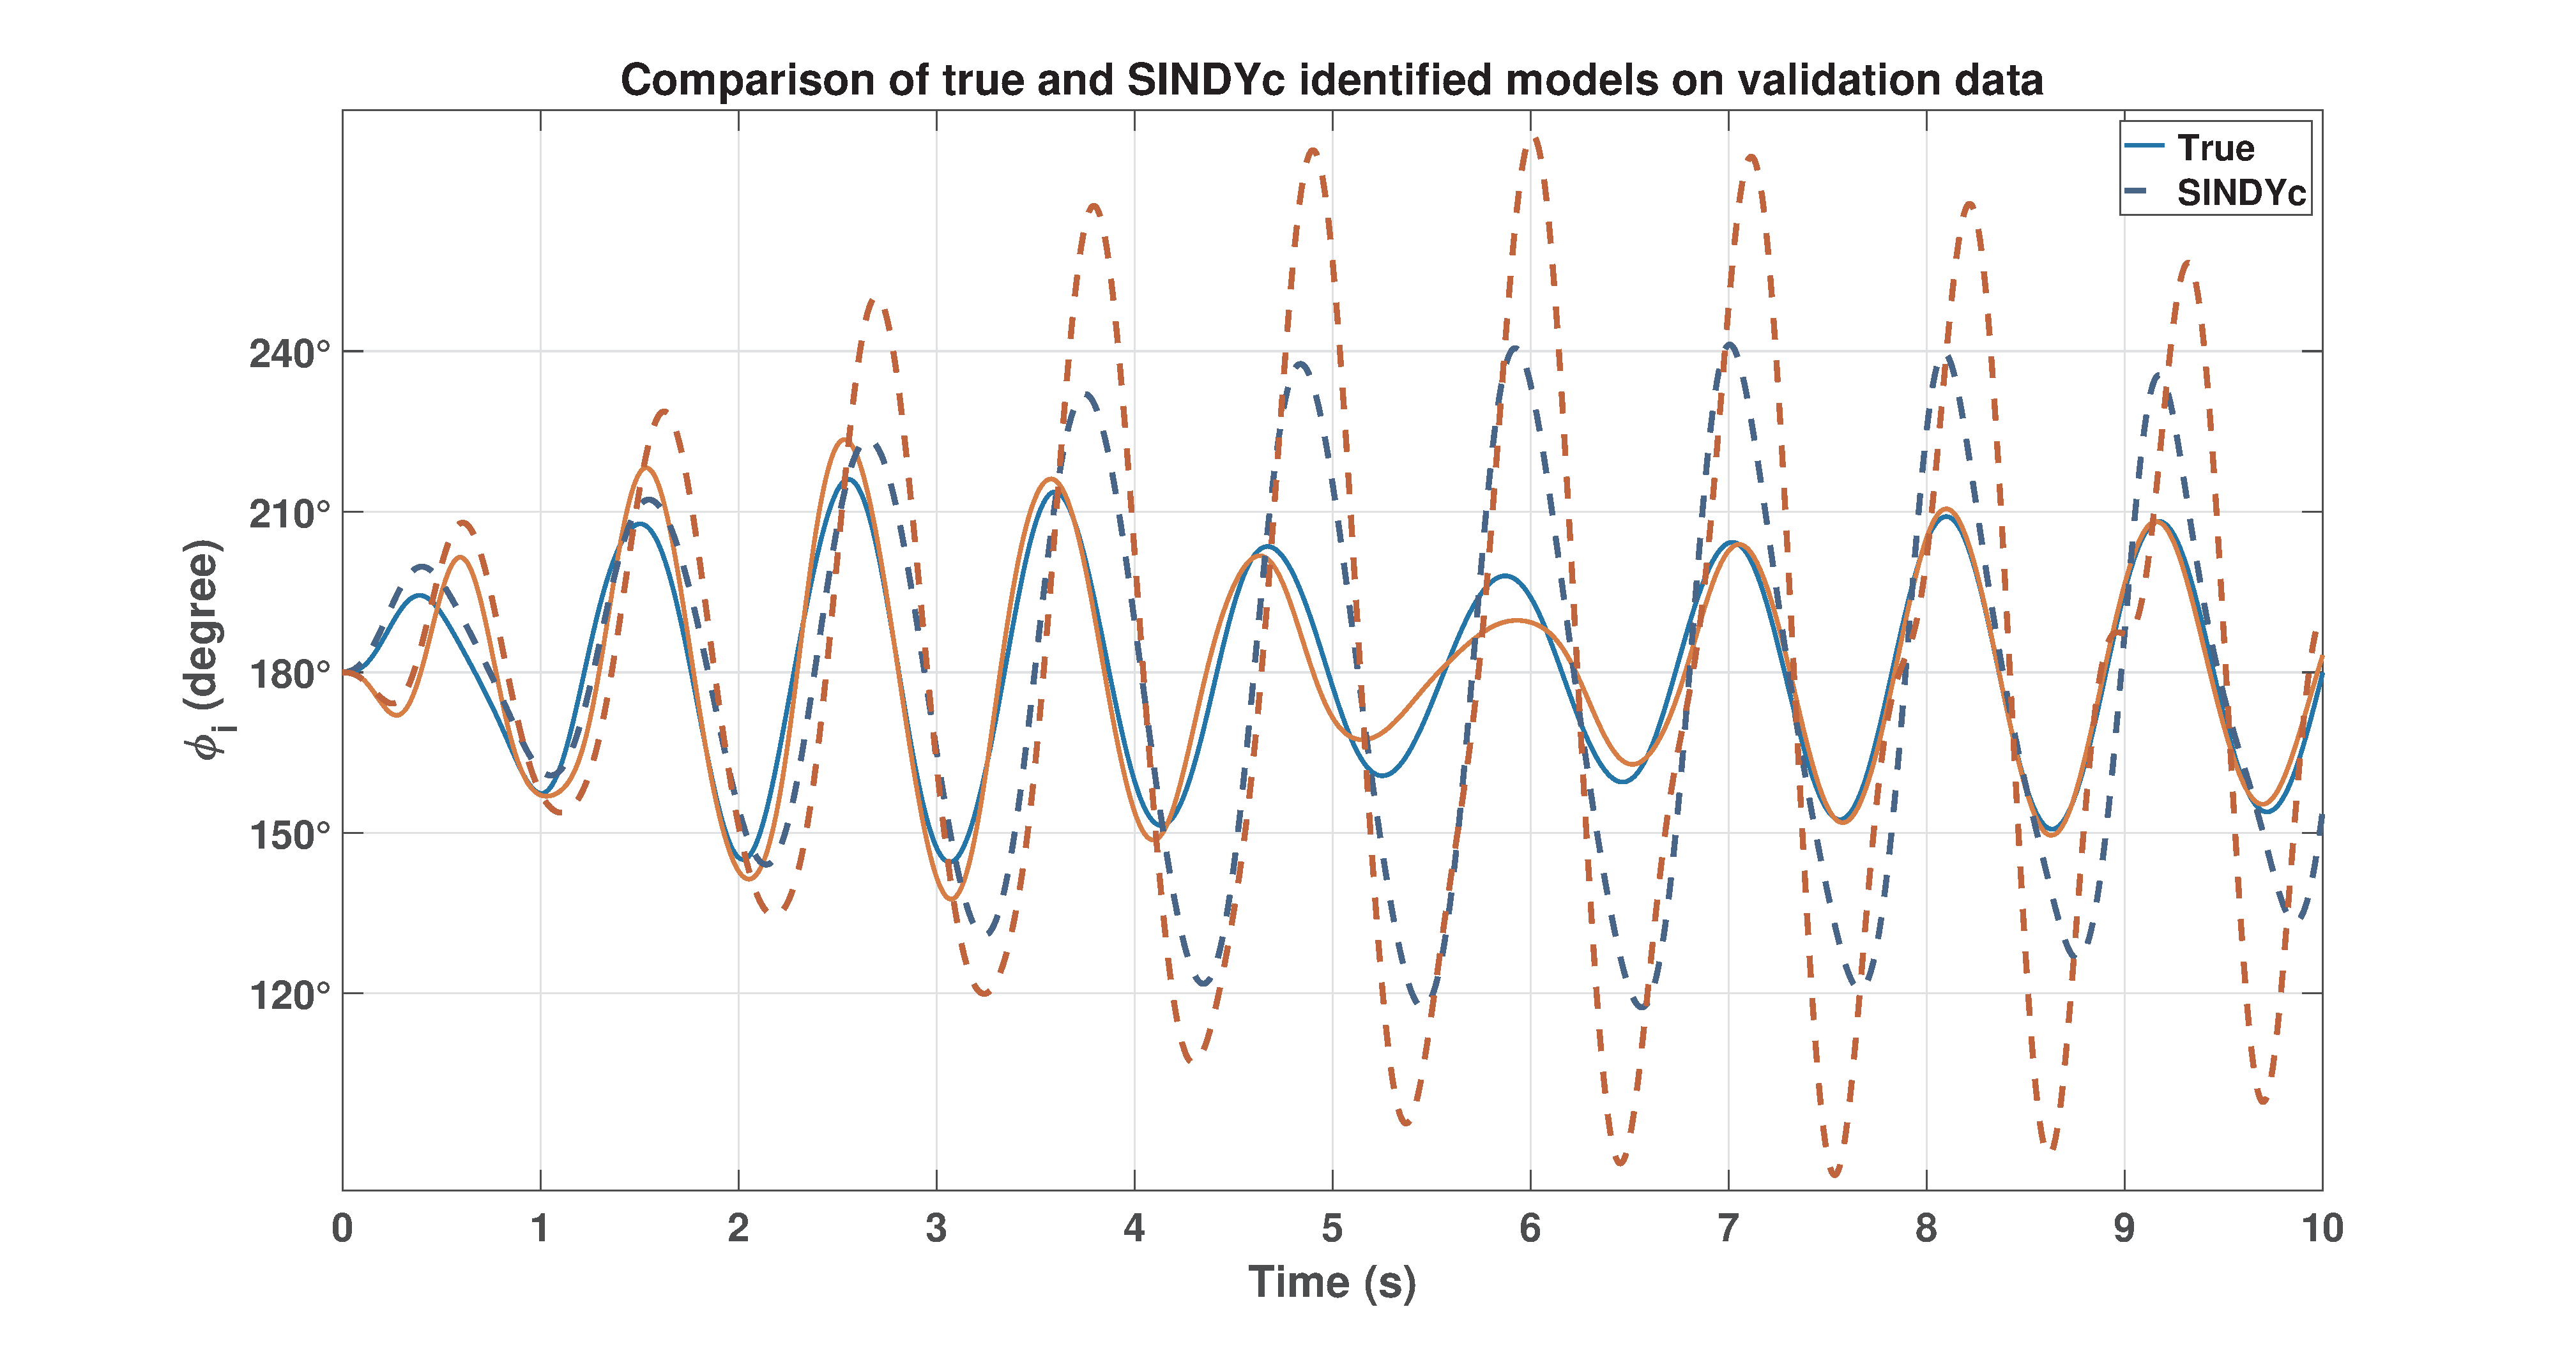
\includegraphics[width=1\linewidth]{figures/MultTrajVal_2_0_0}
    \caption{Identification with multiple trajectories and $\mathbf{\Psi_2}$ on validation data}
    \label{fig: MultTrajVal2}
\end{figure}
% 
The following section applies the knowledge obtained from this section to efficiently synthesize a data-driven controller for the ADIP to track a closed-loop reference trajectory.\newpage